\documentclass{article}
\usepackage[utf8]{inputenc}
\usepackage{graphicx}
\pagenumbering{gobble}
\usepackage{tikz}
\usetikzlibrary{calc}
\usetikzlibrary{positioning}


\usepackage{geometry}
 \geometry{
 a4paper,
 total={170mm,257mm},
 left=20mm,
 top=20mm,
 }



\begin{document}


\begin{figure}
\centering    
\textbf{\scriptsize{a)}}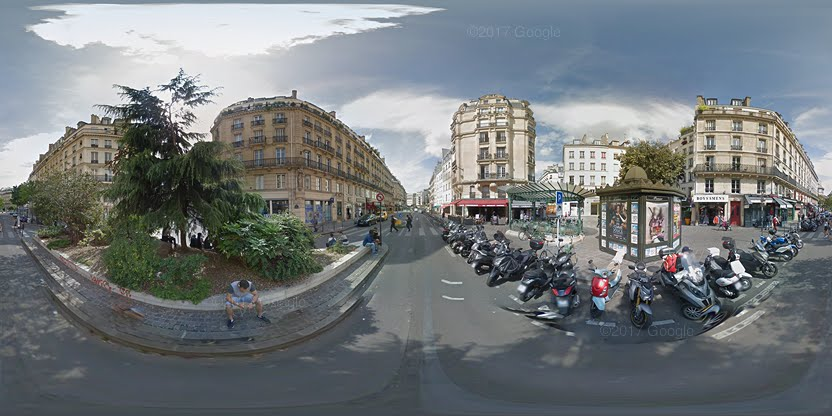
\includegraphics[scale=0.25]{Images/2/panorama-JtVHmEl7WCiz1xJ0bcJpBg-1.png} 
\textbf{\scriptsize{c)}}\includegraphics[scale=0.22]{Images/2/20130902_123654_cropped.png} 
\textbf{\scriptsize{b)}}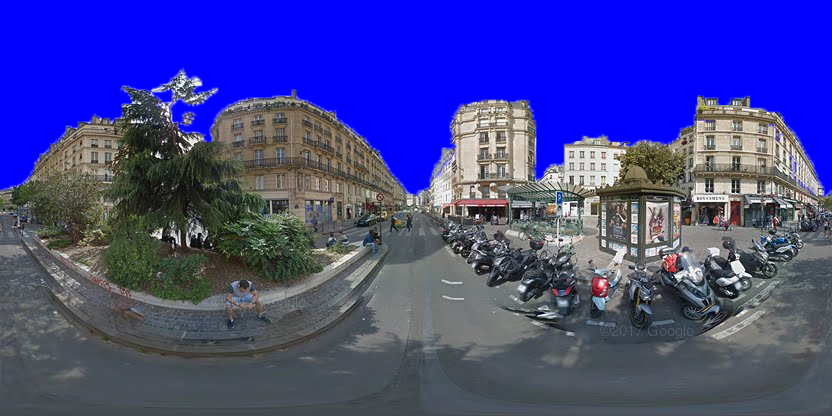
\includegraphics[scale=0.25]{Images/2/panorama-JtVHmEl7WCiz1xJ0bcJpBg-1-marked.png} 
\textbf{\scriptsize{d)}}\includegraphics[scale=0.22]{Images/2/19106.png} 
%\caption{\bf a) Original GSV panorama image and b) hand-marked validation image. c) Original Skyfinder image and d) Skyfinder validation mask.}    
 \label{fig:origmarked}  
\end{figure} 



\clearpage %1


\begin{figure}
\centering    
\textbf{\scriptsize{a)}}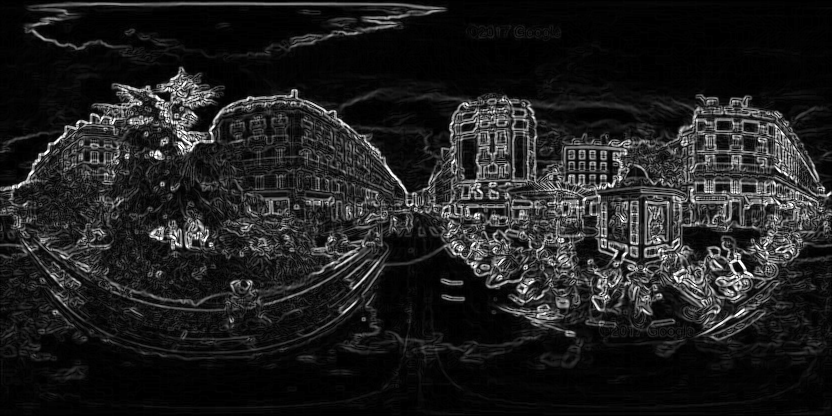
\includegraphics[scale=0.24]{Images/2/panorama-JtVHmEl7WCiz1xJ0bcJpBg-1_Sobel.png} 
\textbf{\scriptsize{b)}}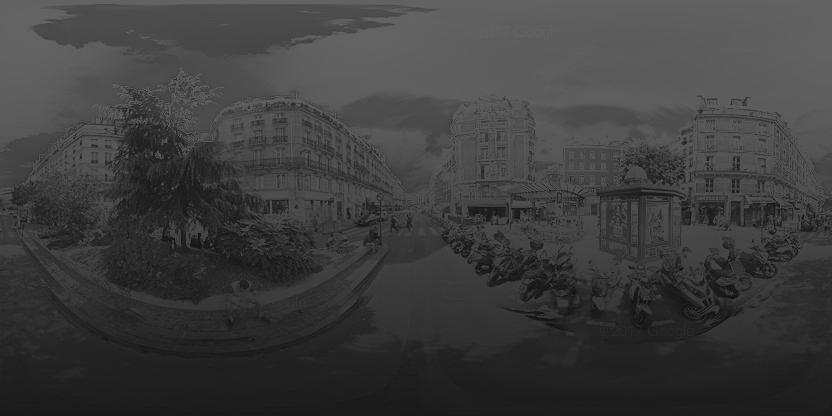
\includegraphics[scale=0.24]{Images/2/panorama-JtVHmEl7WCiz1xJ0bcJpBg-1_Sobel_prob.png} 
\textbf{\scriptsize{c)}}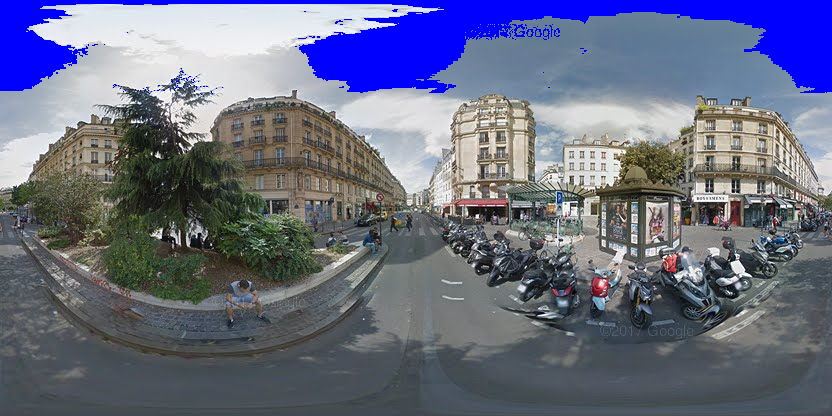
\includegraphics[scale=0.24]{Images/2/panorama-JtVHmEl7WCiz1xJ0bcJpBg-1_Sobel_95_marked.png} 
\textbf{\scriptsize{d)}}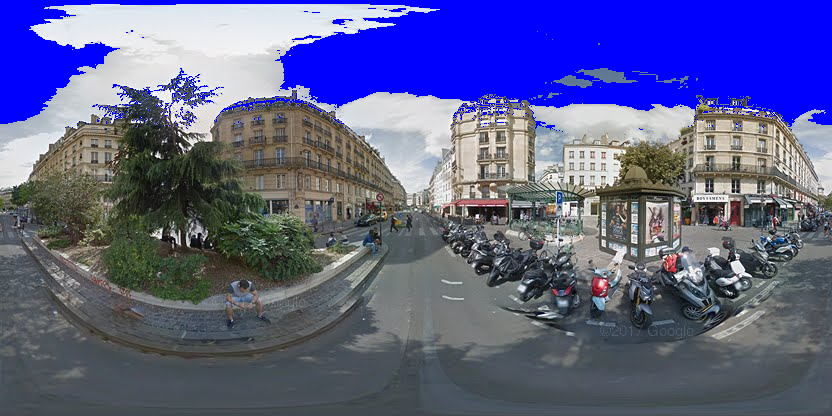
\includegraphics[scale=0.24]{Images/2/panorama-JtVHmEl7WCiz1xJ0bcJpBg-1_Sobel_90_marked.png} 
\textbf{\scriptsize{e)}}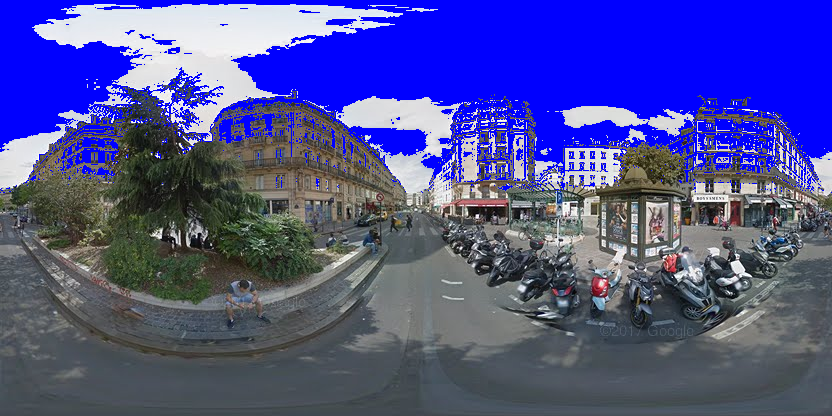
\includegraphics[scale=0.24]{Images/2/panorama-JtVHmEl7WCiz1xJ0bcJpBg-1_Sobel_80_marked.png} 
\textbf{\scriptsize{f)}}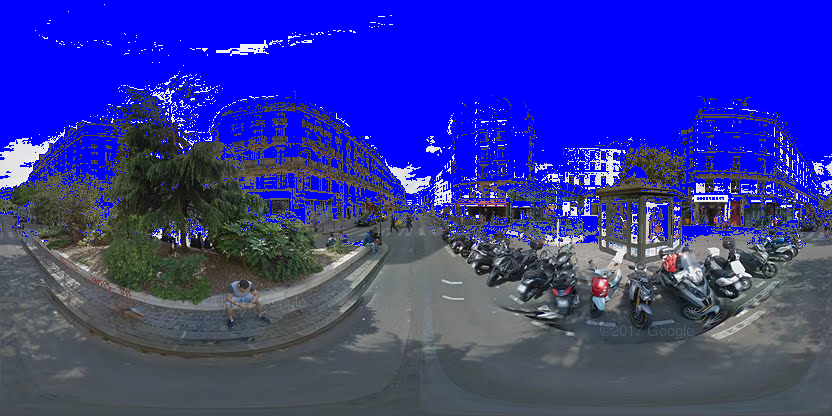
\includegraphics[scale=0.24]{Images/2/panorama-JtVHmEl7WCiz1xJ0bcJpBg-1_Sobel_70_marked.png} 
\textbf{\scriptsize{g)}}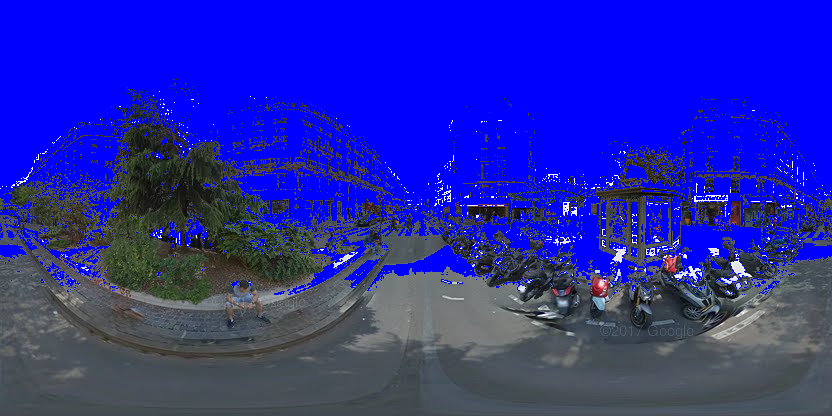
\includegraphics[scale=0.24]{Images/2/panorama-JtVHmEl7WCiz1xJ0bcJpBg-1_Sobel_60_marked.png} 
\textbf{\scriptsize{h)}}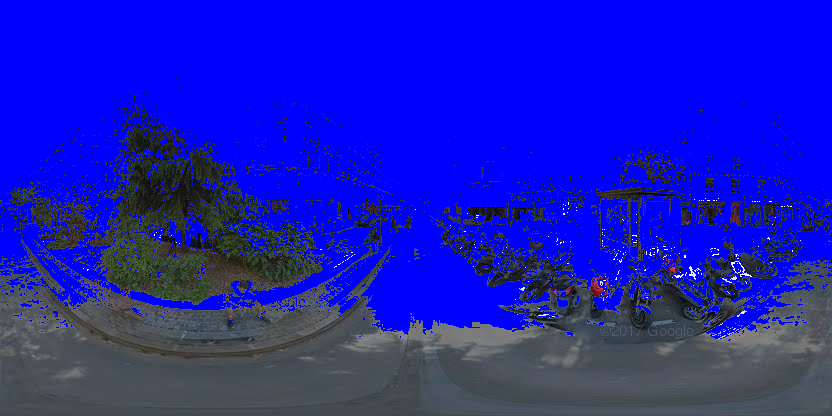
\includegraphics[scale=0.24]{Images/2/panorama-JtVHmEl7WCiz1xJ0bcJpBg-1_Sobel_50_marked.png} 
%\caption{\bf  Results of Sobel operator/hybrid probability model, showing a) Sobel operator gradient image, b) resulting probability predictions, c) Sobel\_50, d) Sobel\_60, e) Sobel\_70, f) Sobel\_80, g) Sobel\_90, and h) Sobel\_95.}    
 %\label{fig:sobolresults}  
\end{figure} 

\clearpage %2

\begin{figure}
\centering    
\textbf{\phantom{\textbf{\scriptsize{a)}}}}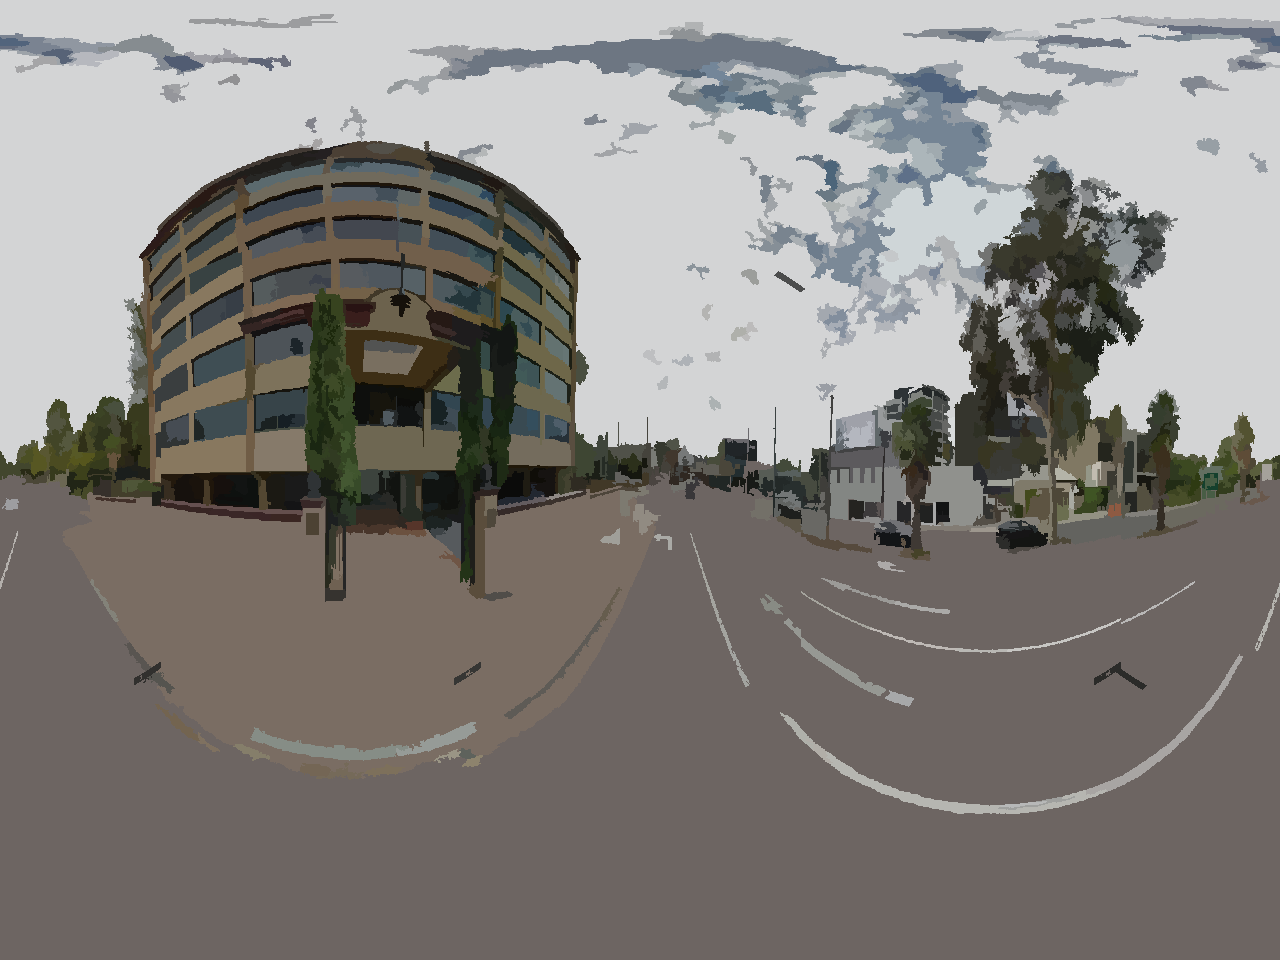
\includegraphics[scale=0.08]{Images/mean/4880_3_6_100.png} 
\textbf{\phantom{\textbf{\scriptsize{b)}}}}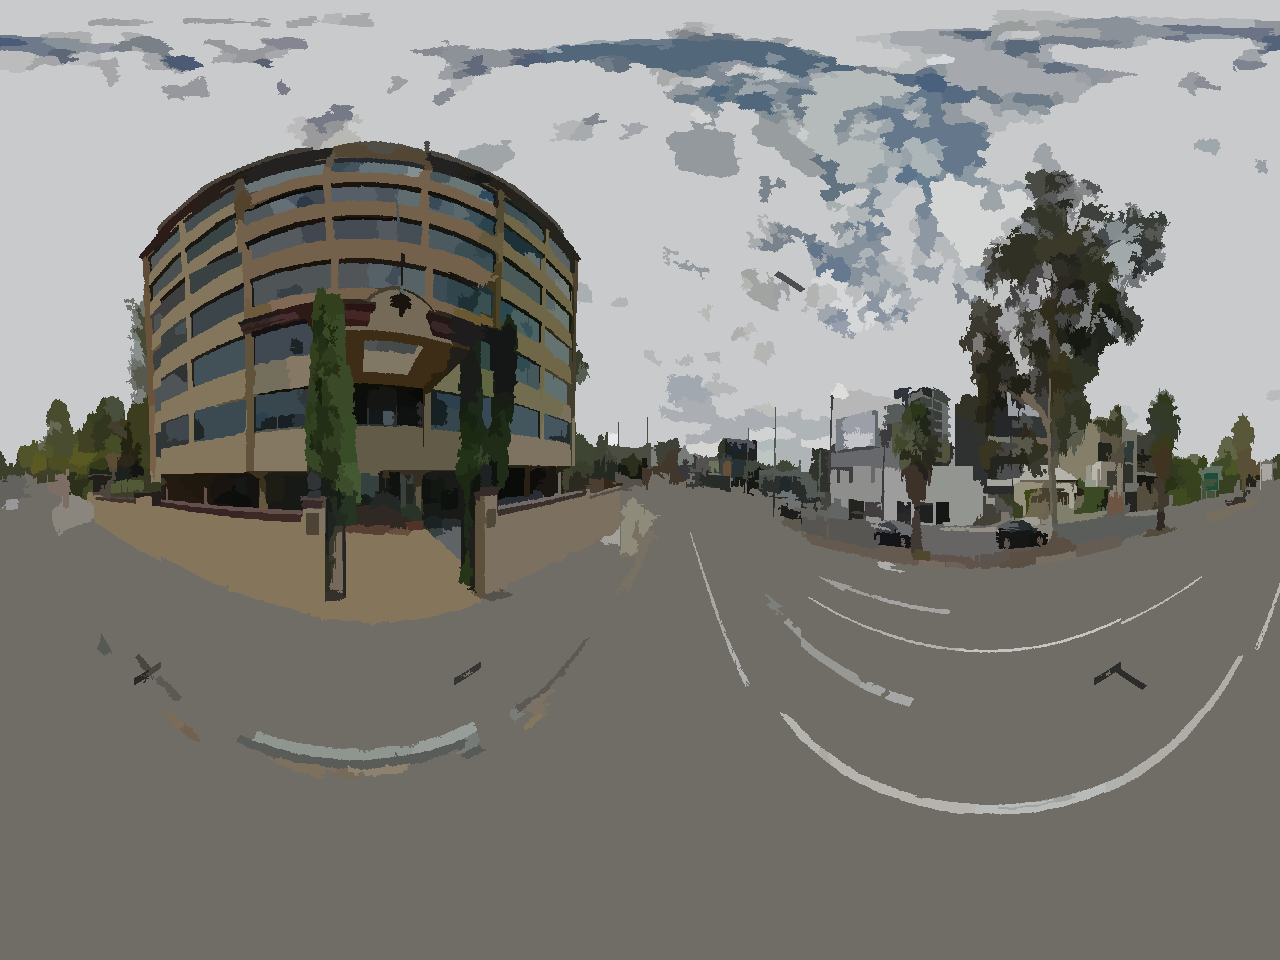
\includegraphics[scale=0.08]{Images/mean/4880_7_6_100.png} 
\textbf{\phantom{\textbf{\scriptsize{c)}}}}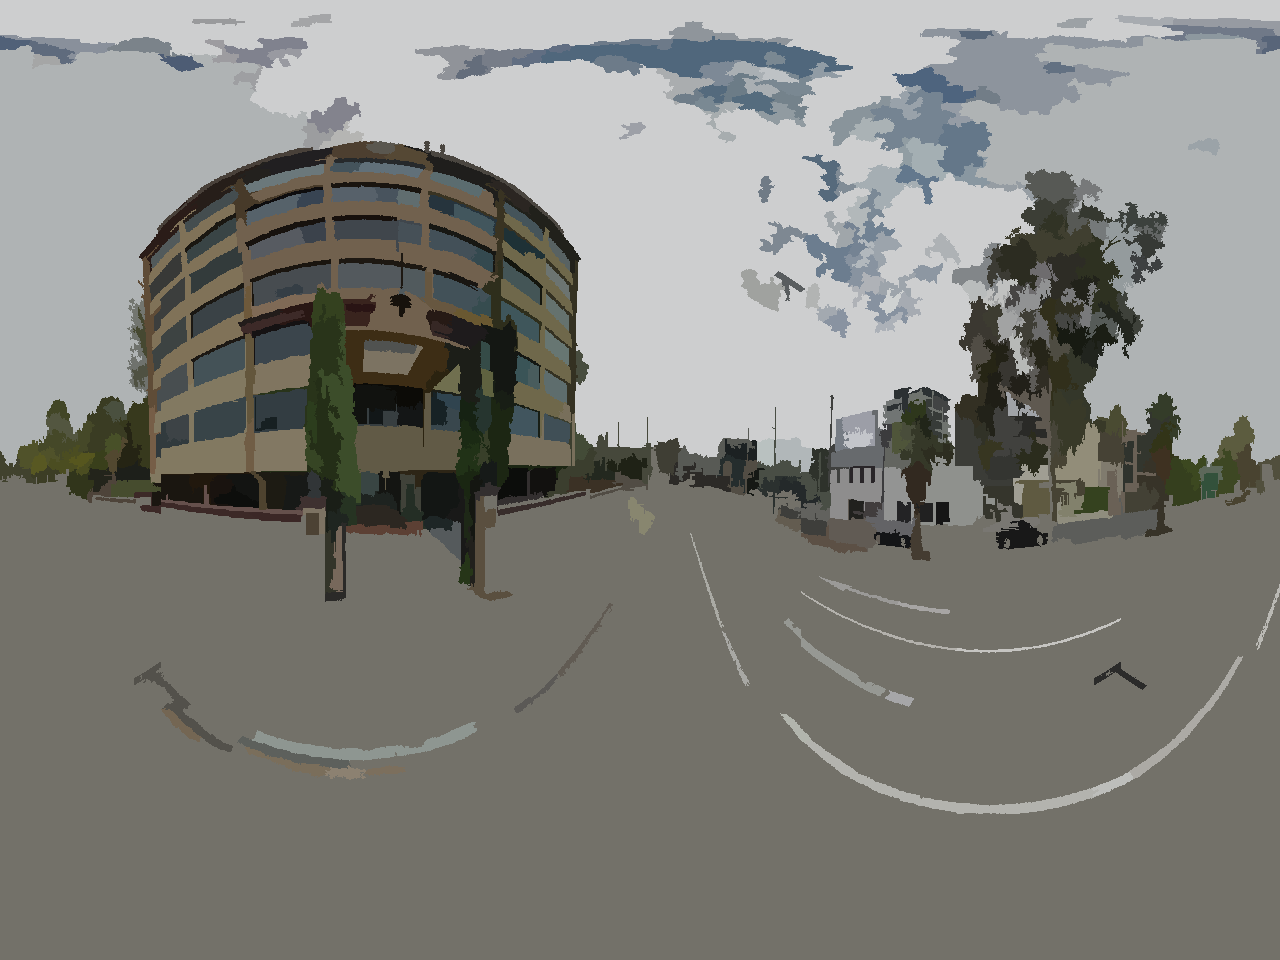
\includegraphics[scale=0.08]{Images/mean/4880_5_7_210.png} 
\textbf{\phantom{\textbf{\scriptsize{d)}}}}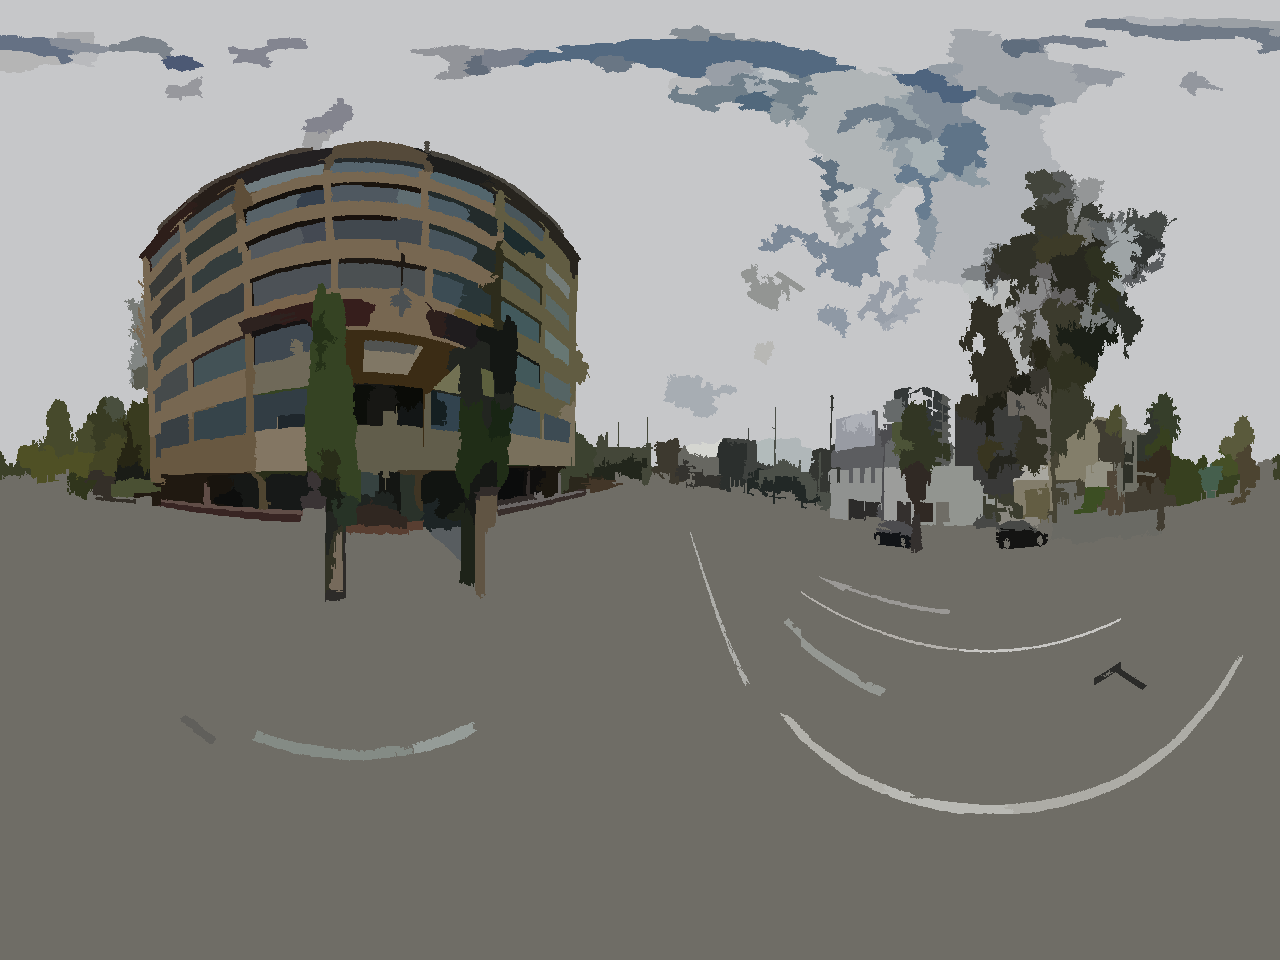
\includegraphics[scale=0.08]{Images/mean/4880_7_8_300.png} \scriptsize{1)}
\textbf{\phantom{\textbf{\scriptsize{a)}}}}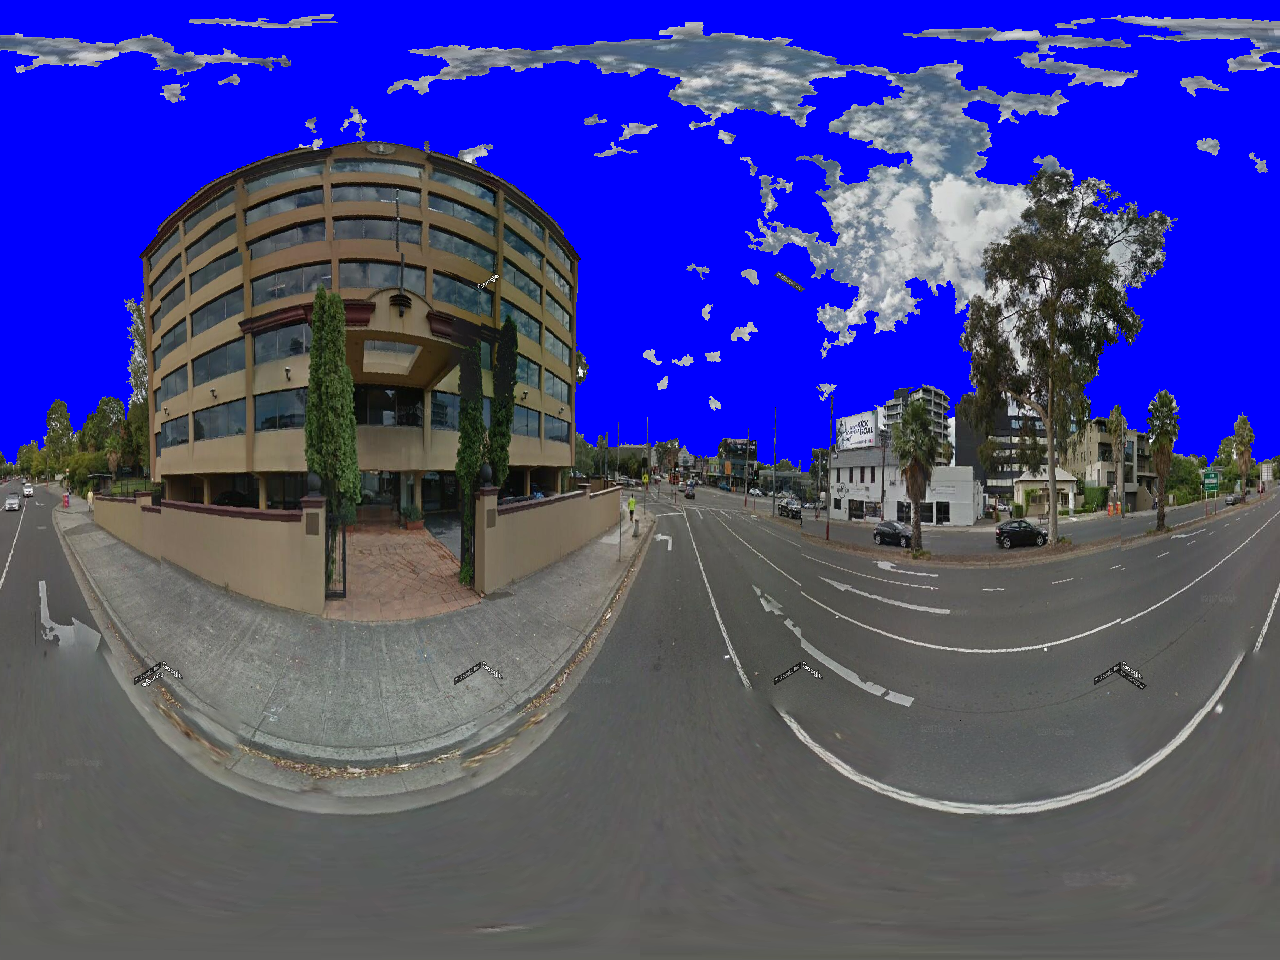
\includegraphics[scale=0.08]{Images/mean/4880_3_6_100_ms_sky_mark.png} 
\textbf{\phantom{\textbf{\scriptsize{b)}}}}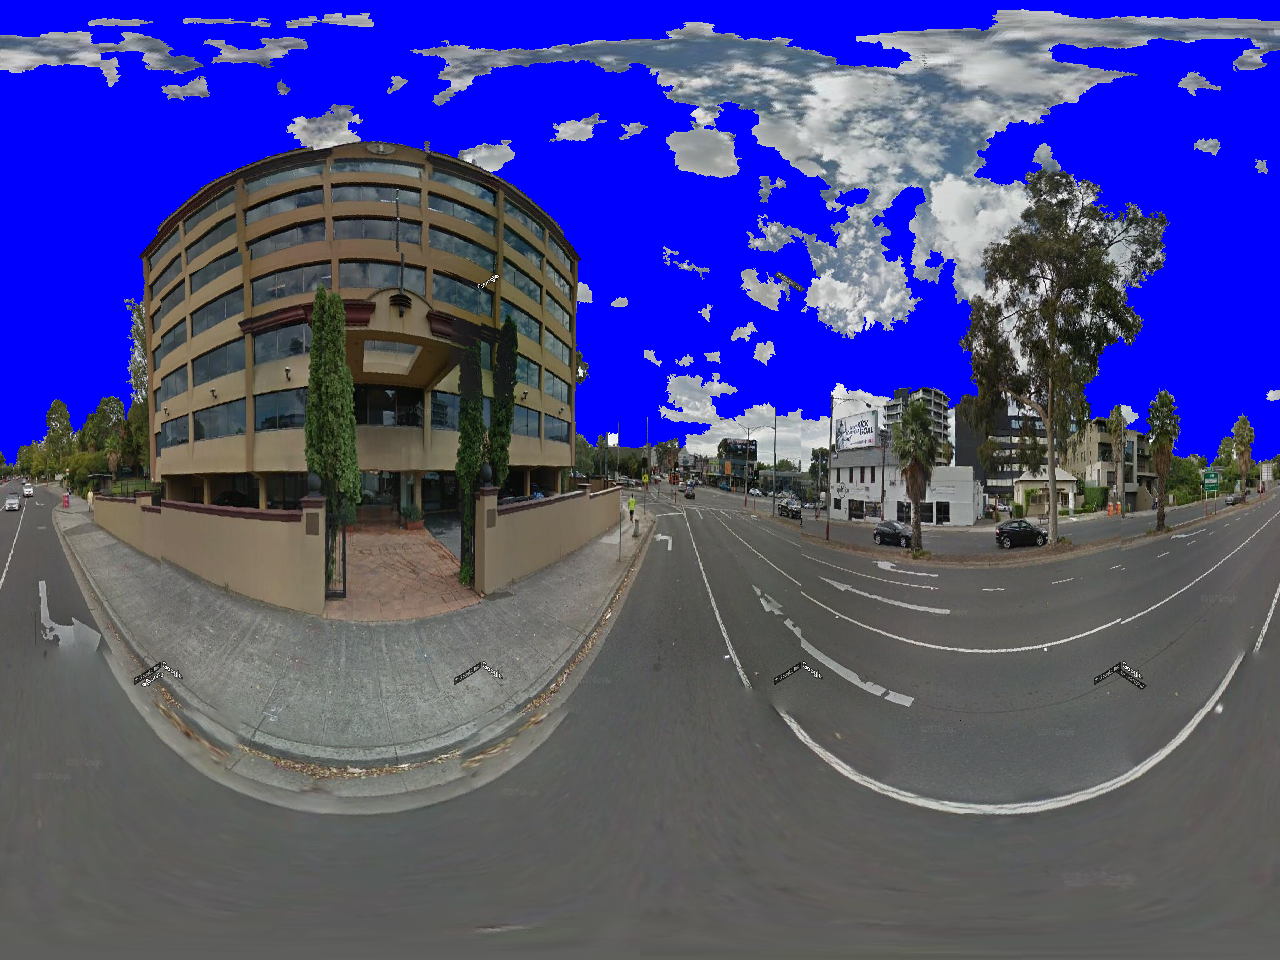
\includegraphics[scale=0.08]{Images/mean/4880_7_6_100_ms_sky_mark.png} 
\textbf{\phantom{\textbf{\scriptsize{c)}}}}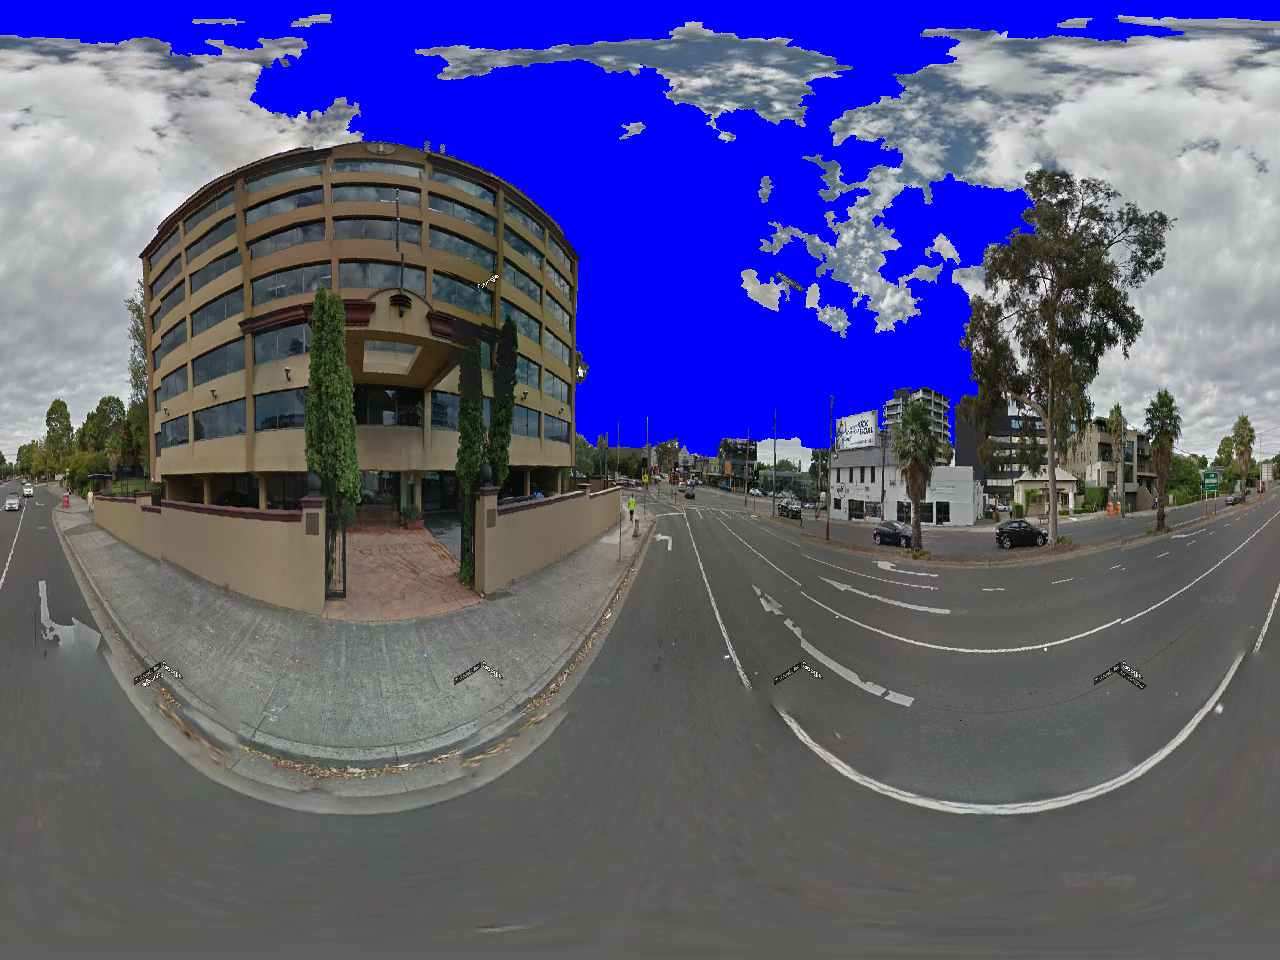
\includegraphics[scale=0.08]{Images/mean/4880_5_7_210_ms_sky_mark.png} 
\textbf{\phantom{\textbf{\scriptsize{d)}}}}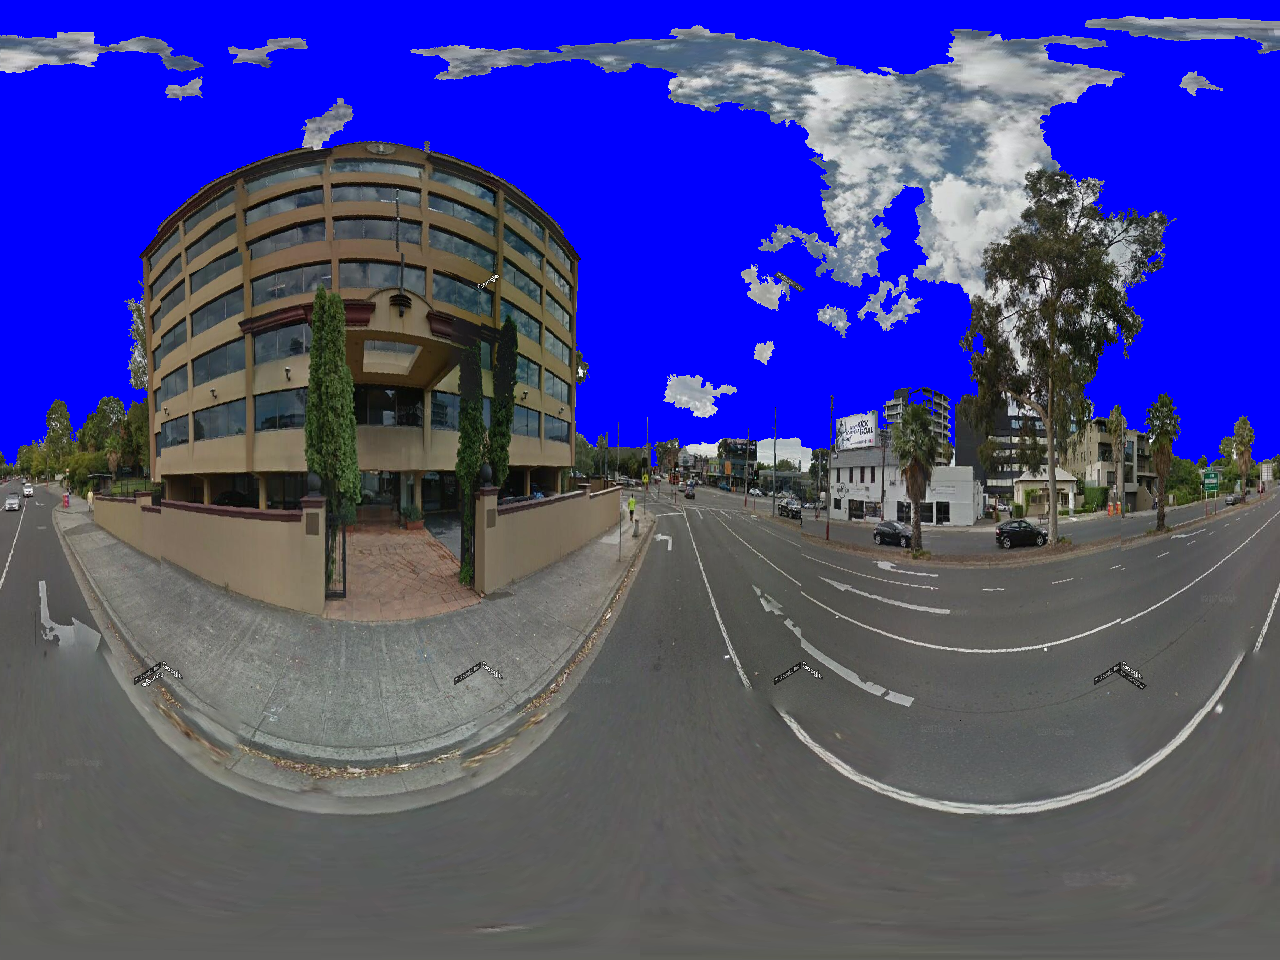
\includegraphics[scale=0.08]{Images/mean/4880_7_8_300_ms_sky_mark.png} \scriptsize{2)}
%\textbf{\phantom{\textbf{\scriptsize{a)}}}}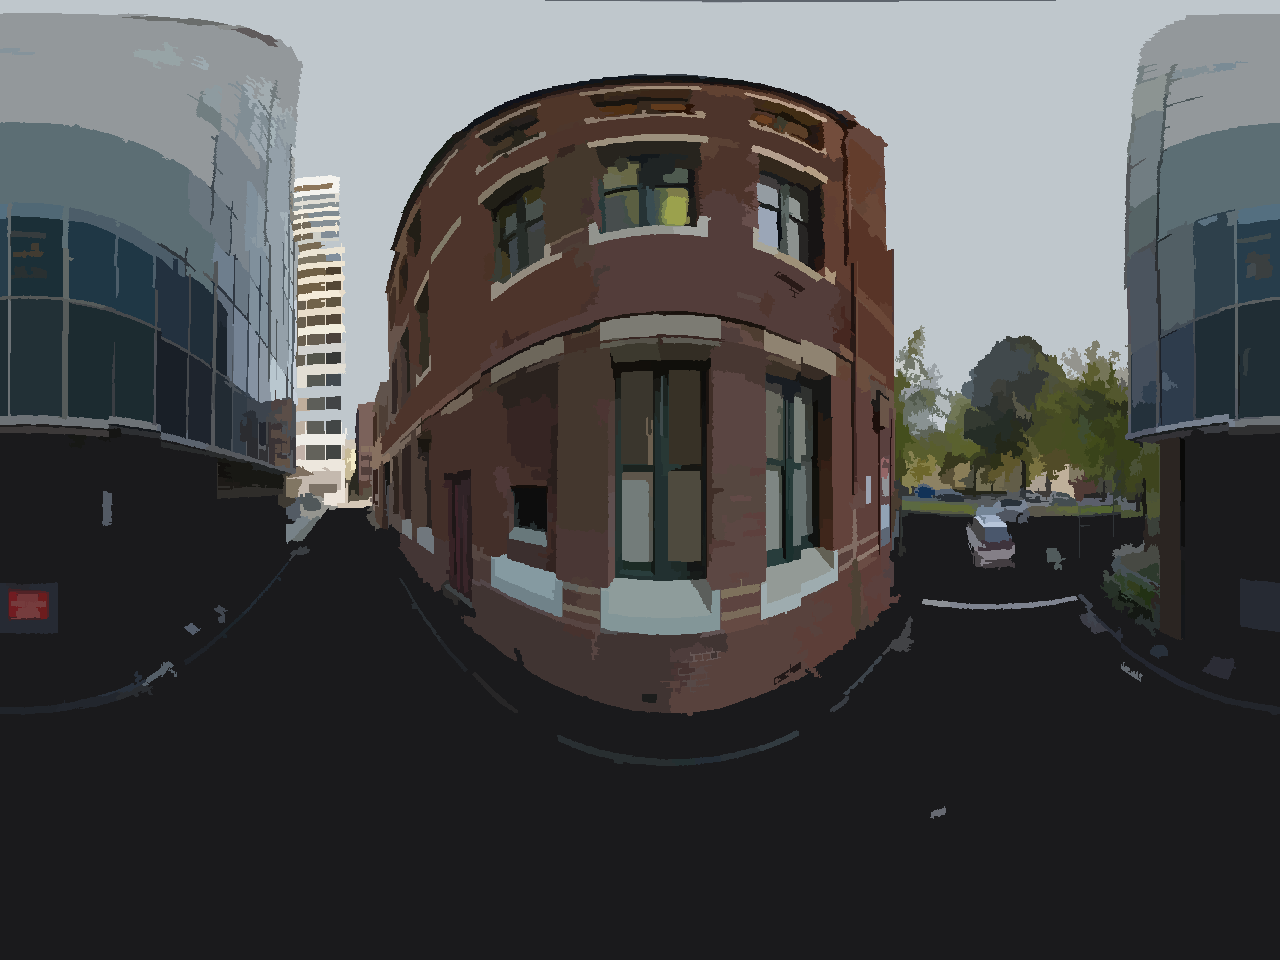
\includegraphics[scale=0.08]{Images/mean/0070_3_6_100.png} 
\textbf{\phantom{\textbf{\scriptsize{a)}}}}\includegraphics[scale=0.08]{/home/kerryn/git/2018-03-MasterITProject/SkyViewDetection/SkyfinderEvaluationOutput/GSV2/mark_output_BigBuilding_3_6.0_100/0070_panorama_seg.png} 
%\textbf{\phantom{\textbf{\scriptsize{b)}}}}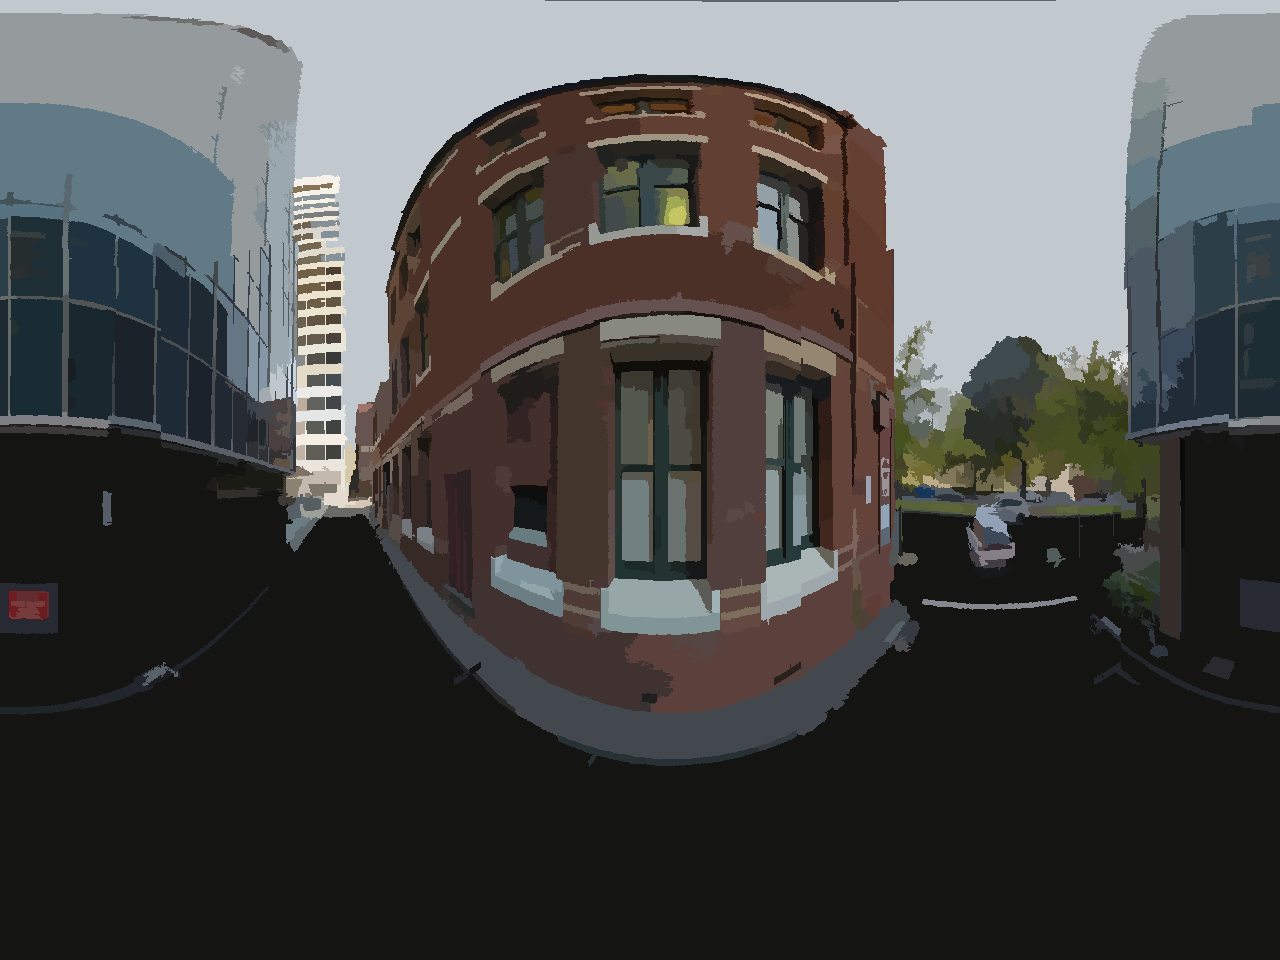
\includegraphics[scale=0.08]{Images/mean/0070_7_6_100.png} 
\textbf{\phantom{\textbf{\scriptsize{b)}}}}\includegraphics[scale=0.08]{/home/kerryn/git/2018-03-MasterITProject/SkyViewDetection/SkyfinderEvaluationOutput/GSV2/mark_output_BigBuilding_7_6.0_100/0070_panorama_seg.png} 
%\textbf{\phantom{\textbf{\scriptsize{c)}}}}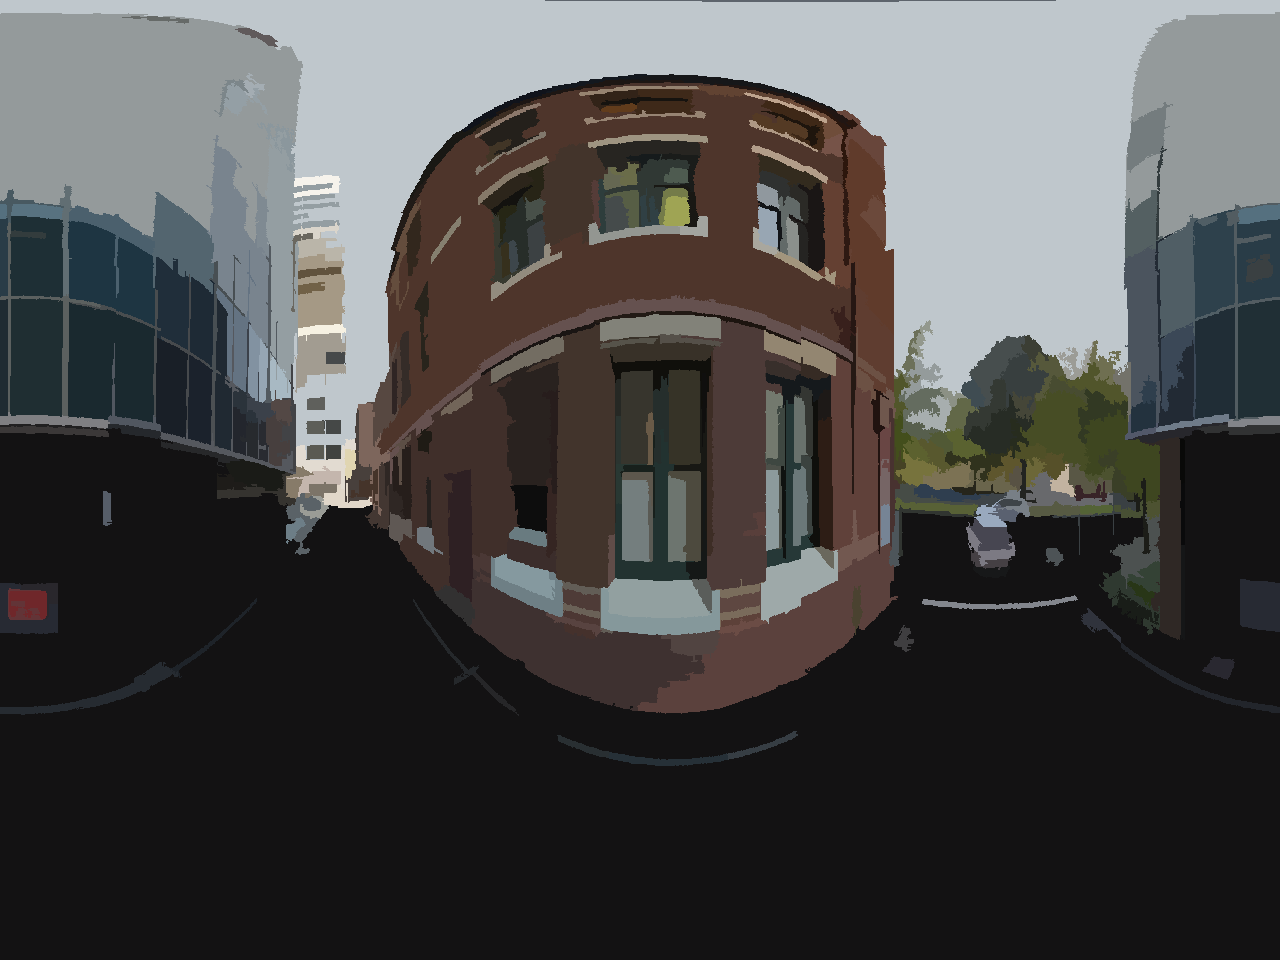
\includegraphics[scale=0.08]{Images/mean/0070_5_7_210.png} 
\textbf{\phantom{\textbf{\scriptsize{c)}}}}\includegraphics[scale=0.08]{/home/kerryn/git/2018-03-MasterITProject/SkyViewDetection/SkyfinderEvaluationOutput/GSV2/mark_output_BigBuilding_5_7.0_210/0070_panorama_seg.png} 
%\textbf{\phantom{\textbf{\scriptsize{d)}}}}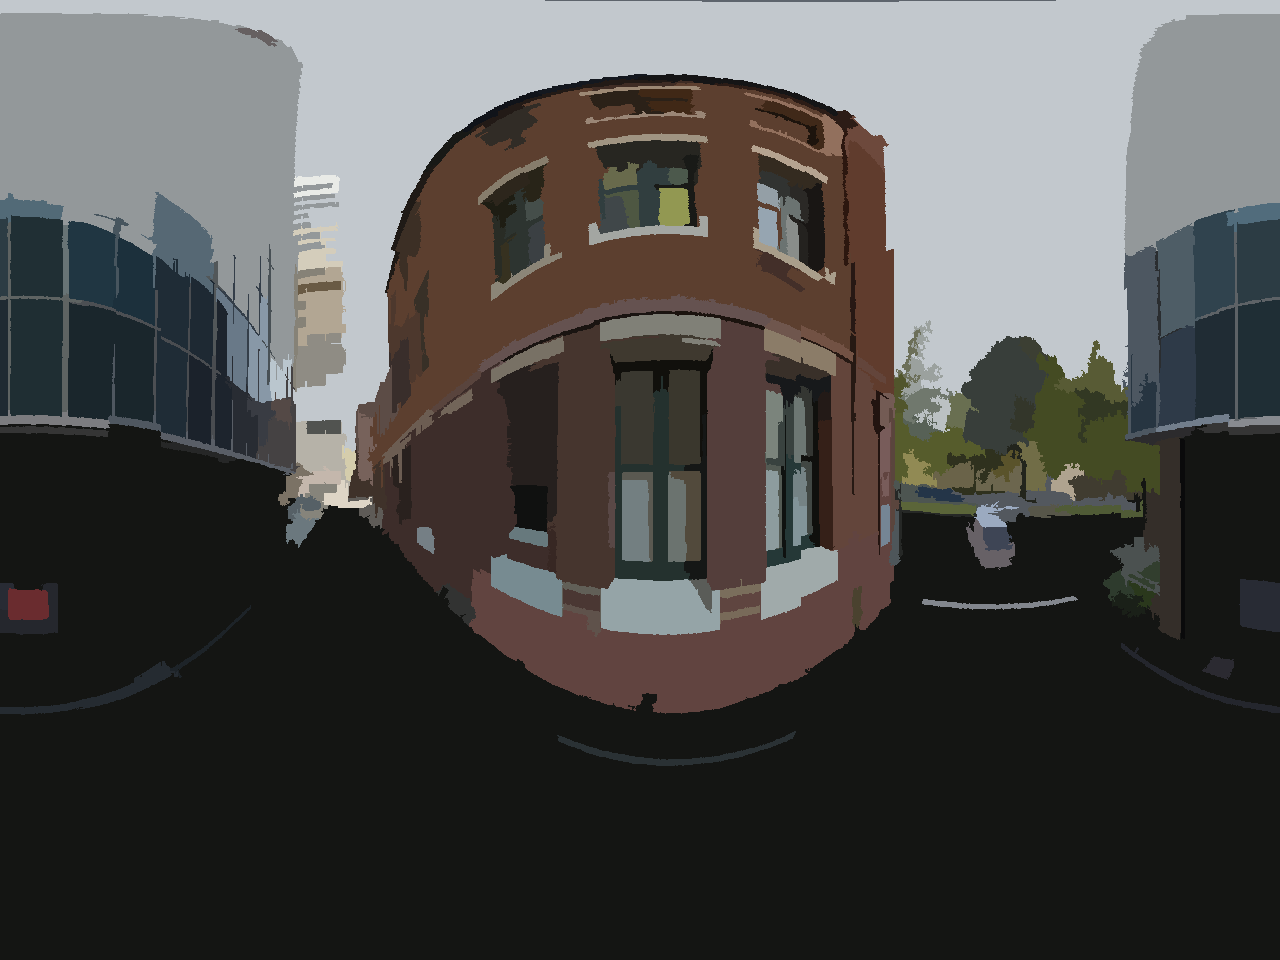
\includegraphics[scale=0.08]{Images/mean/0070_7_8_300.png} \scriptsize{3)}
\textbf{\phantom{\textbf{\scriptsize{d)}}}}\includegraphics[scale=0.08]{/home/kerryn/git/2018-03-MasterITProject/SkyViewDetection/SkyfinderEvaluationOutput/GSV2/mark_output_BigBuilding/0070_panorama_seg.png} \scriptsize{3)}
%\textbf{\scriptsize{a)}}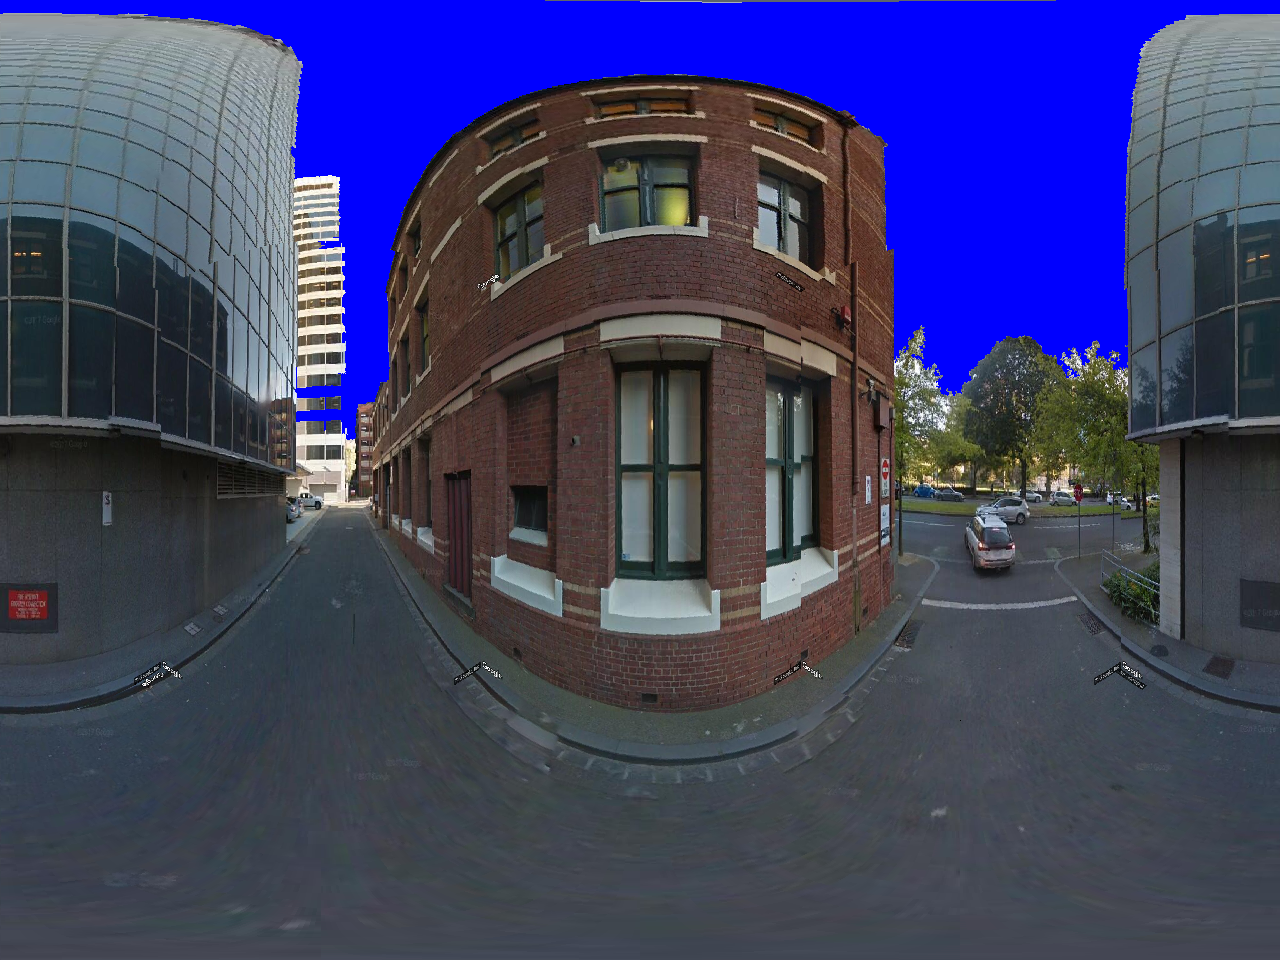
\includegraphics[scale=0.08]{Images/mean/0070_3_6_100_ms_sky_mark.png} 
\textbf{\scriptsize{a)}}\includegraphics[scale=0.08]{/home/kerryn/git/2018-03-MasterITProject/SkyViewDetection/SkyfinderEvaluationOutput/GSV2/mark_output_BigBuilding_3_6.0_100/0070_panorama_ms_sky_mark.png} 
%\textbf{\scriptsize{b)}}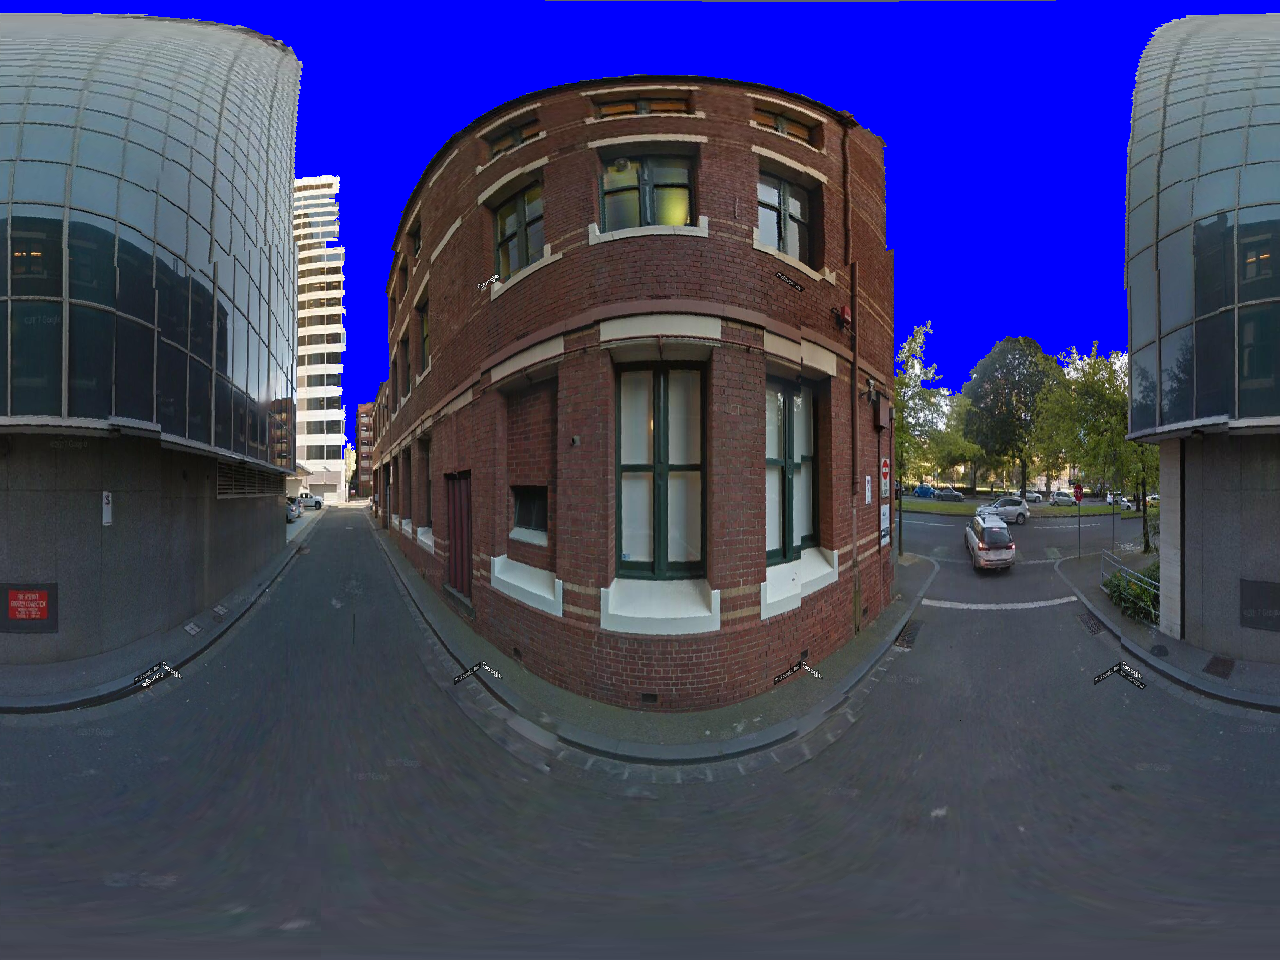
\includegraphics[scale=0.08]{Images/mean/0070_7_6_100_ms_sky_mark.png} 
\textbf{\scriptsize{b)}}\includegraphics[scale=0.08]{/home/kerryn/git/2018-03-MasterITProject/SkyViewDetection/SkyfinderEvaluationOutput/GSV2/mark_output_BigBuilding_7_6.0_100/0070_panorama_ms_sky_mark.png} 
%\textbf{\scriptsize{c)}}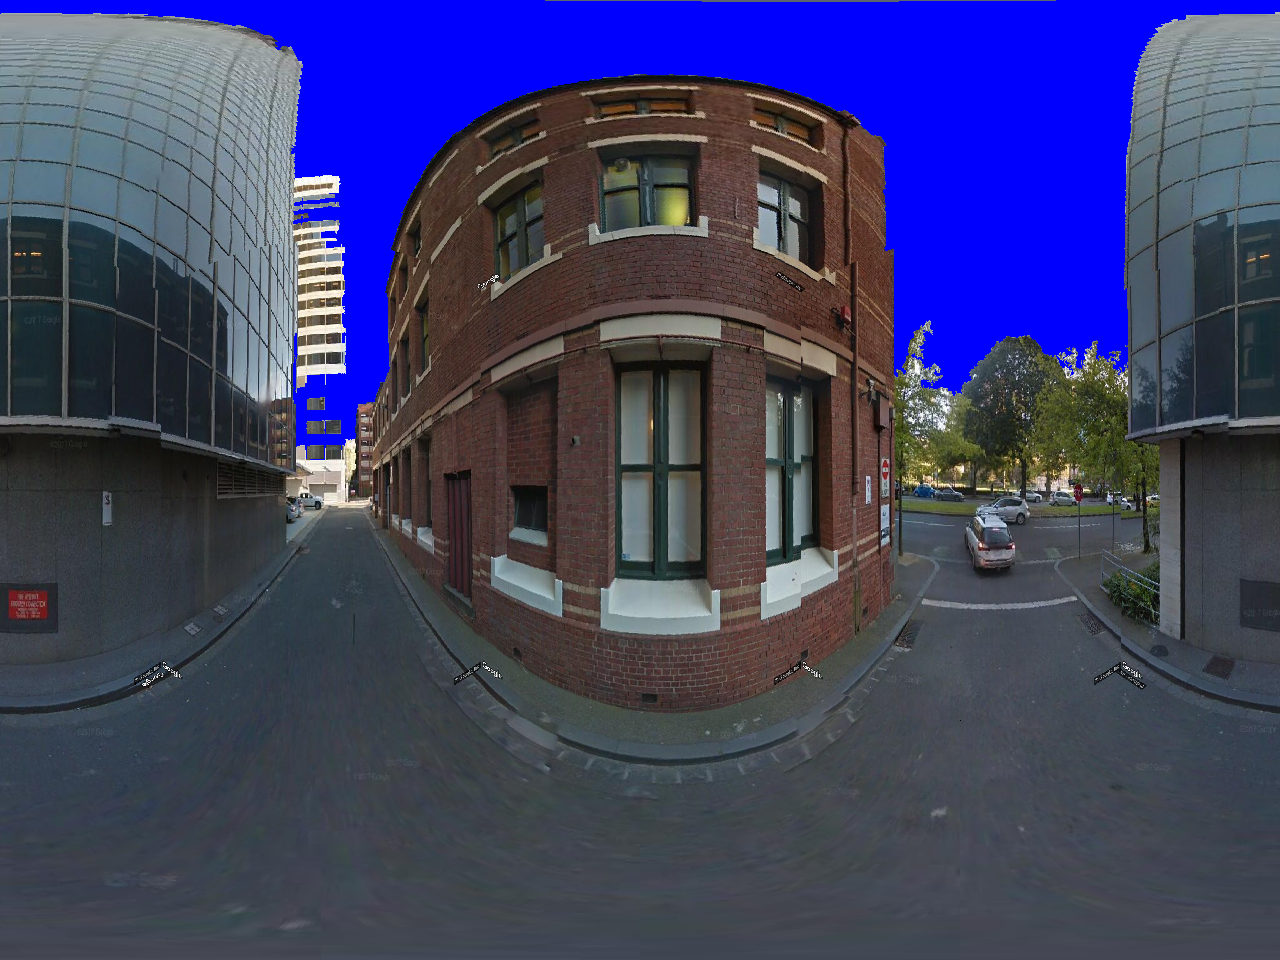
\includegraphics[scale=0.08]{Images/mean/0070_5_7_210_ms_sky_mark.png} 
\textbf{\scriptsize{c)}}\includegraphics[scale=0.08]{/home/kerryn/git/2018-03-MasterITProject/SkyViewDetection/SkyfinderEvaluationOutput/GSV2/mark_output_BigBuilding_5_7.0_210/0070_panorama_ms_sky_mark.png} 
%\textbf{\scriptsize{d)}}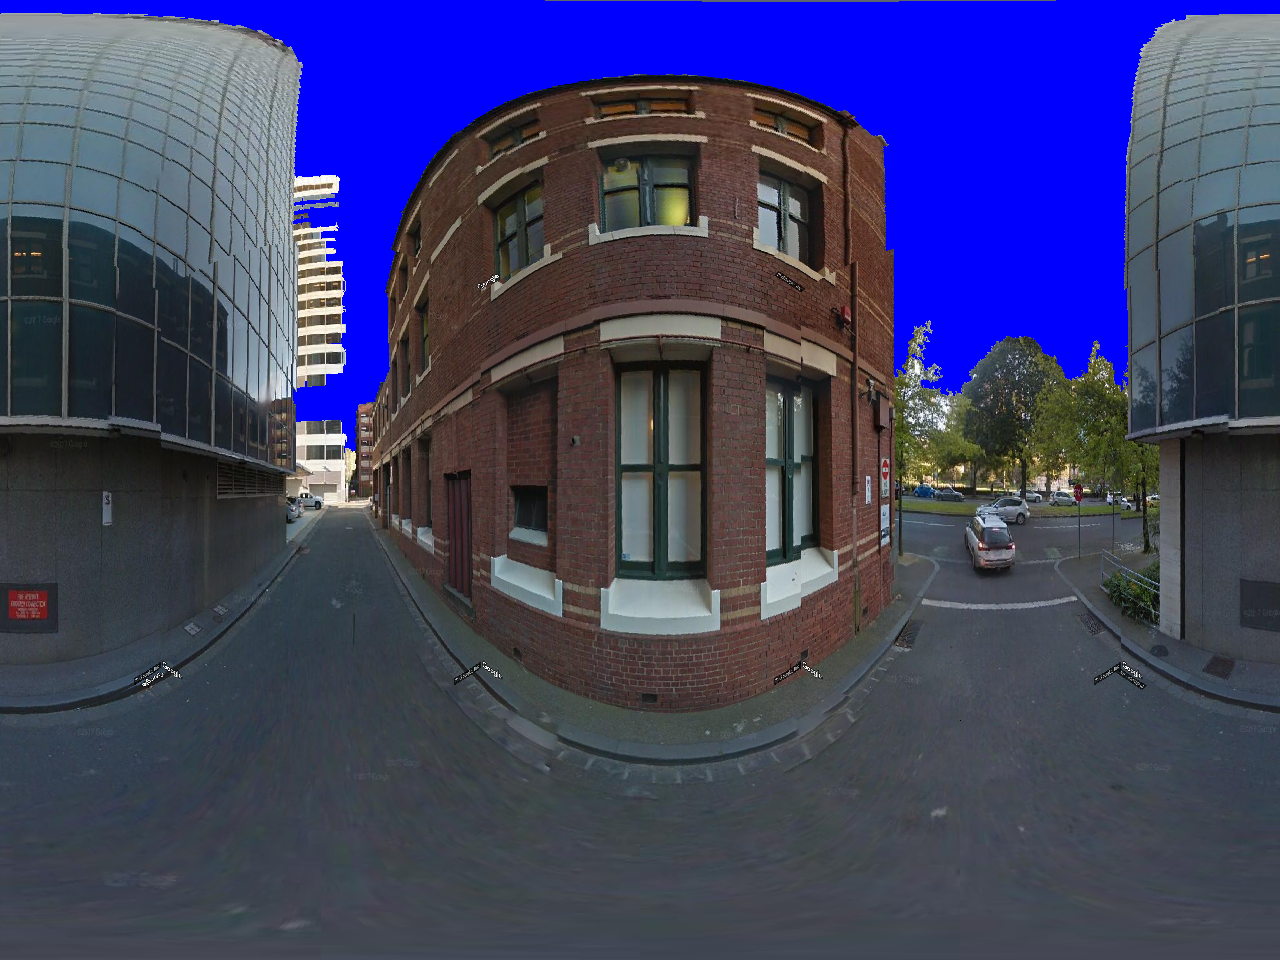
\includegraphics[scale=0.08]{Images/mean/0070_7_8_300_ms_sky_mark.png} \scriptsize{4)}
\textbf{\scriptsize{d)}}\includegraphics[scale=0.08]{/home/kerryn/git/2018-03-MasterITProject/SkyViewDetection/SkyfinderEvaluationOutput/GSV2/mark_output_BigBuilding/0070_panorama_ms_sky_mark.png} \scriptsize{4)}


%\caption{\bf Comparison outputs of intermediate mean shift segmentation algorithm processing steps using varying parameters, showing columns a) Mean\_3\_6\_100, b) Mean\_7\_6\_100, c) Mean\_5\_7\_210, d) Mean\_7\_8\_300 and rows 1) and 3) intermediate mean shifted and rows 2) and 4) the final marked images. }
% \label{fig:meantypes}  
\end{figure} 

\clearpage %3

\begin{figure}
\centering    
\textbf{\scriptsize{a)}}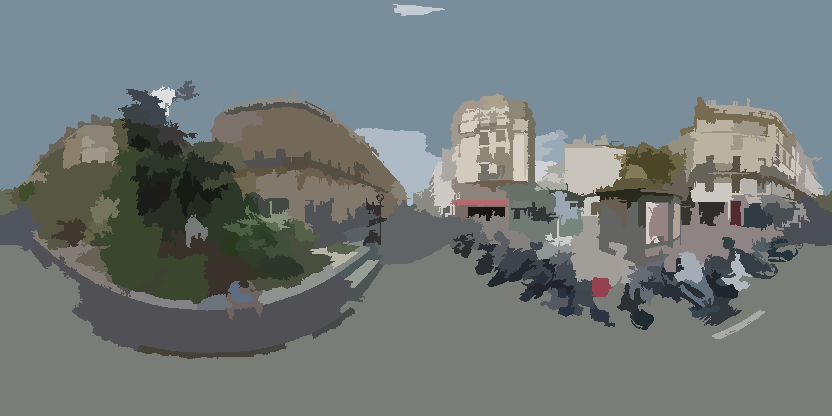
\includegraphics[scale=0.26]{Images/2/panorama-JtVHmEl7WCiz1xJ0bcJpBg-1_seg.png} 
\textbf{\scriptsize{b)}}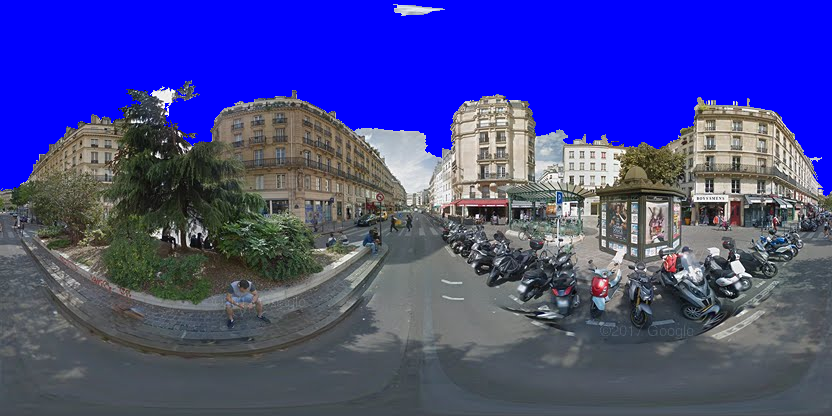
\includegraphics[scale=0.26]{Images/2/panorama-JtVHmEl7WCiz1xJ0bcJpBg-1_ms_sky_mark.png} 
%\caption{\bf Results of mean shift segmentation algorithm (Mean\_5\_7\_210) showing a) mean shifted image and b) final marked image.}    
% \label{fig:meanresults}  
\end{figure} 

\clearpage %4

\begin{figure}
\centering    
%\textbf{a)}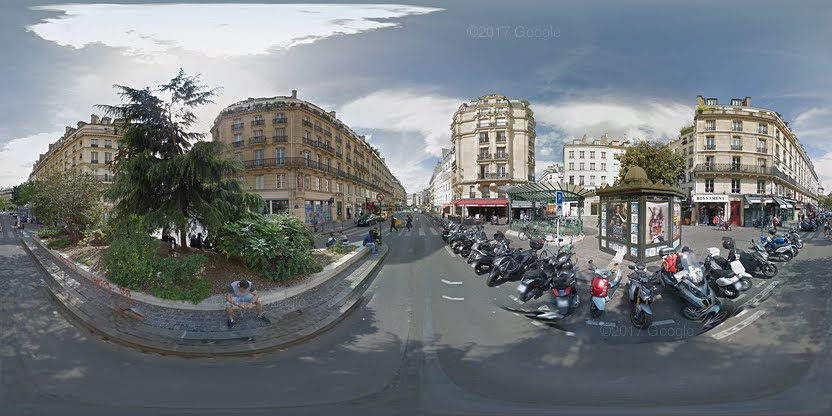
\includegraphics[scale=0.20]{Images/2/Cloudy/panorama-JtVHmEl7WCiz1xJ0bcJpBg-1_cropped.png} 
\textbf{\scriptsize{a)}}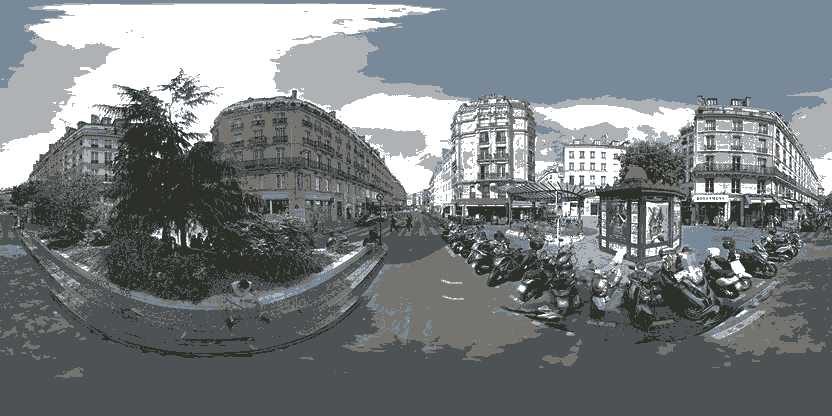
\includegraphics[scale=0.17]{Images/2/Cloudy/panorama-JtVHmEl7WCiz1xJ0bcJpBg-1_clustered6.png} 
\textbf{\scriptsize{b)}}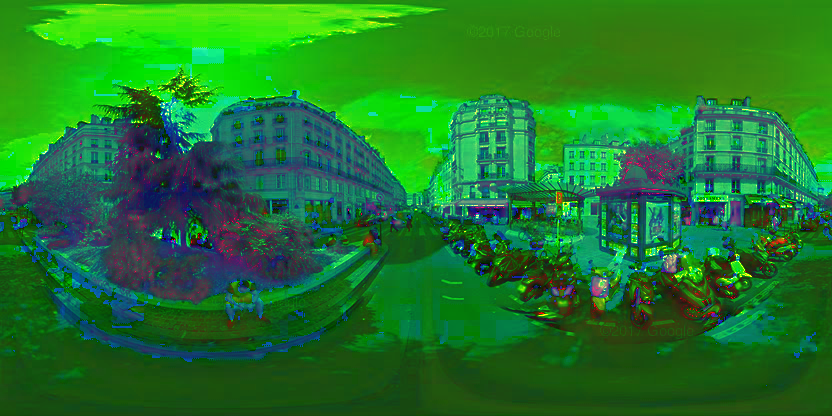
\includegraphics[scale=0.17]{Images/2/Cloudy/panorama-JtVHmEl7WCiz1xJ0bcJpBg-1_HLS6.png} 
\textbf{\scriptsize{c)}}\includegraphics[scale=0.17]{Images/2/Cloudy/{panorama-JtVHmEl7WCiz1xJ0bcJpBg-1_sky_mark0.4}.png} 
%\caption{\bf  Results of K-means clustering and HSL color filtering (K-mean\_6), showing a) K-means clustered image, b) HSL intermediate image, and c) final marked image.}    
% \label{fig:kmeansresults}  
\end{figure} 

\clearpage %5


\begin{figure}
\centering    
\textbf{\scriptsize{a)}}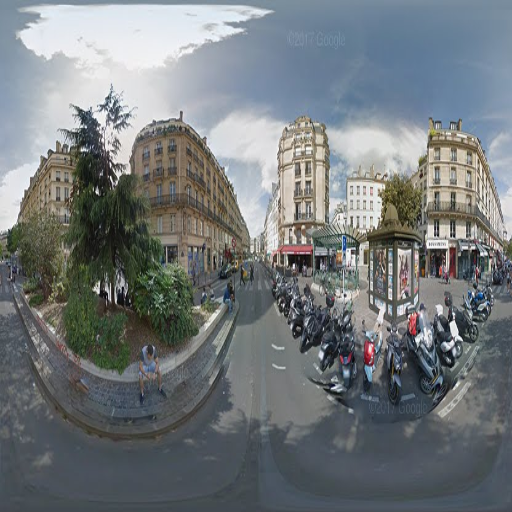
\includegraphics[scale=0.27]{Images/2/FloodfillInput.png}
\textbf{\scriptsize{b)}}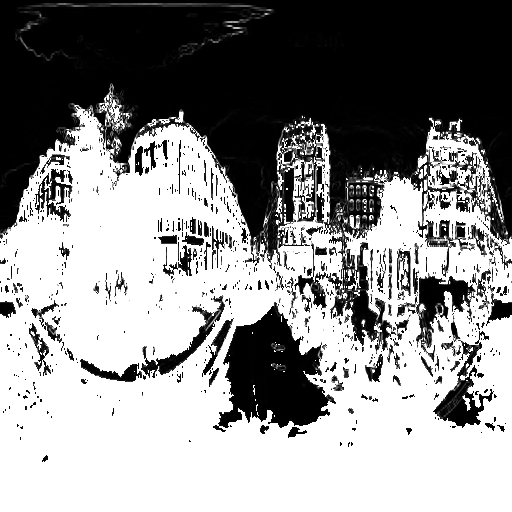
\includegraphics[scale=0.27]{Images/2/FloodfillMiddle.png}
\textbf{\scriptsize{c)}}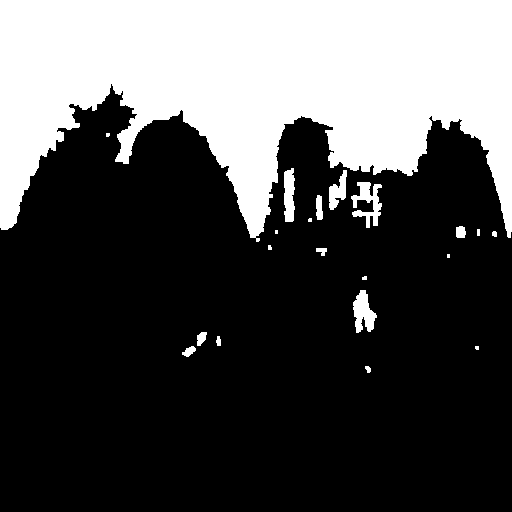
\includegraphics[scale=0.27]{Images/2/FloodfillOutput.png}
%\caption{\bf   Results of Sobel/flood-fill combination, showing a) original image (rescaled to 512x512), b) intermediate Sobel image, and c) final marked sky image.}    
% \label{fig:sobelflood}  
\end{figure} 

\clearpage %6


\begin{figure}
\centering
%\textbf{\scriptsize{a)}}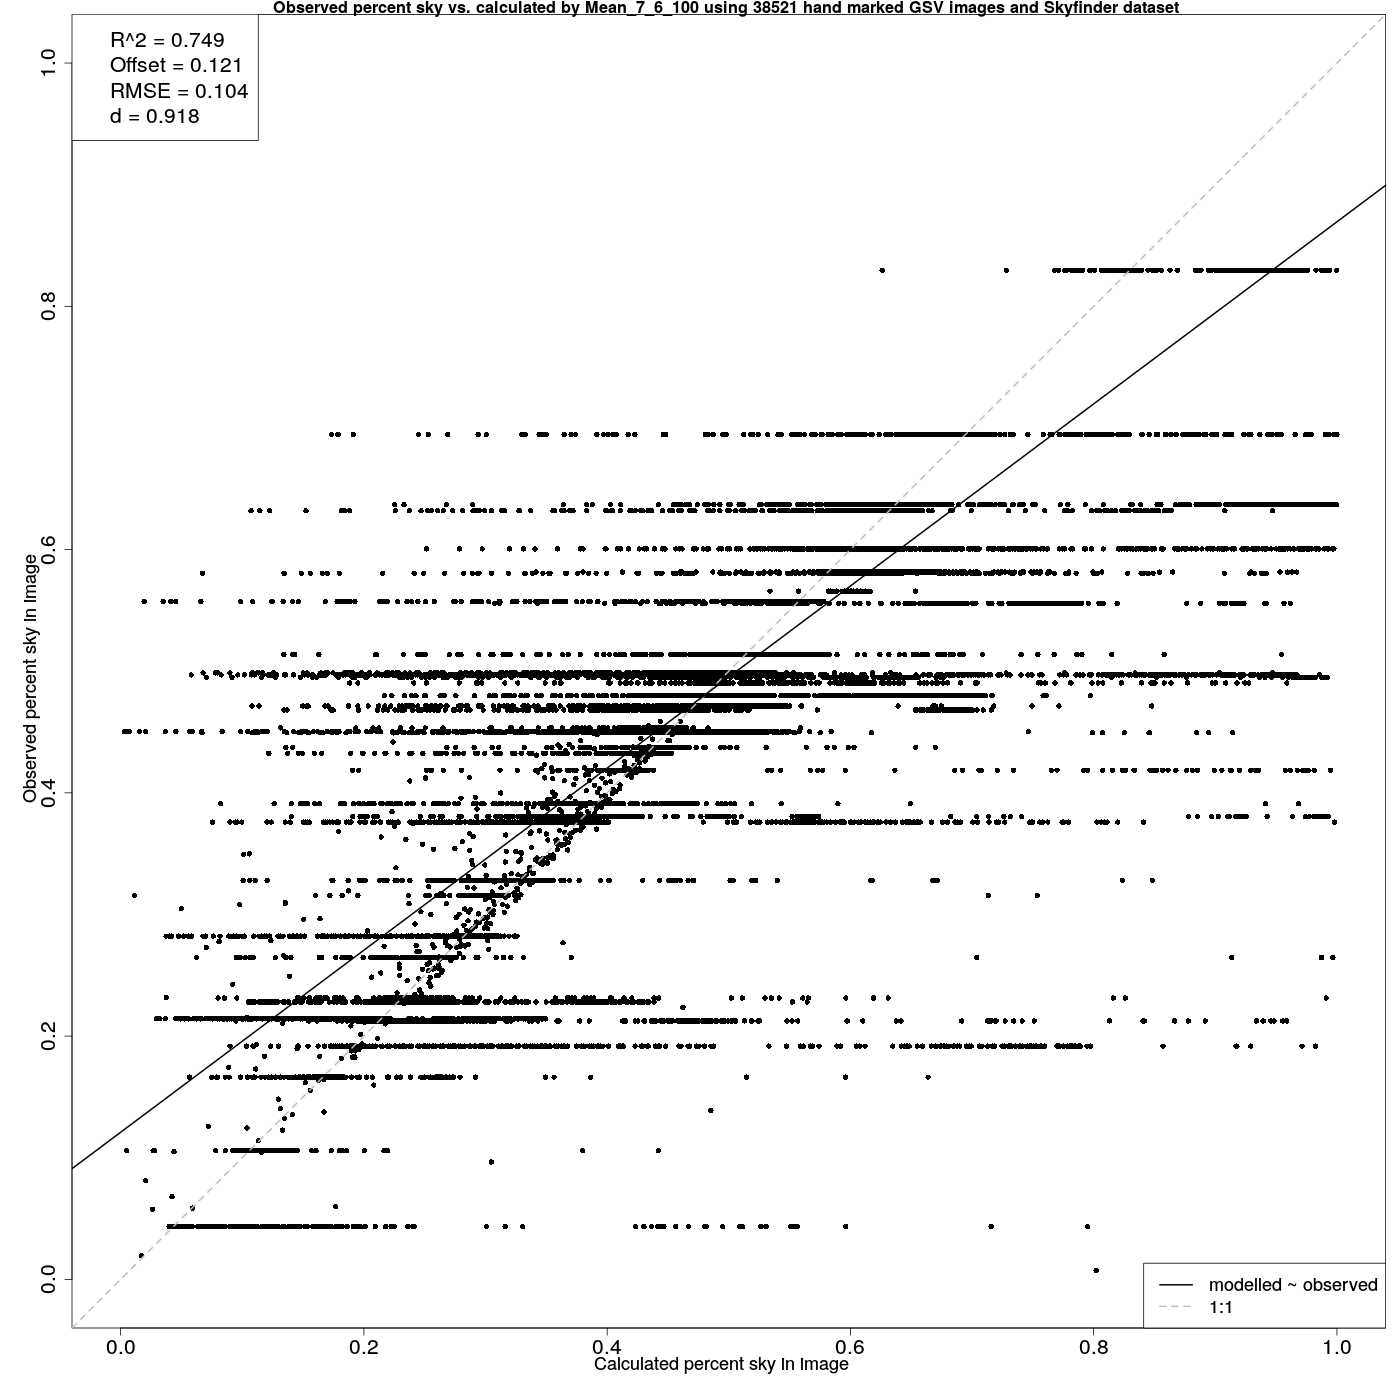
\includegraphics[scale=0.15,trim={8 10 5 0},clip]{Images/ErrorPlotsCombinedIndivMean_7_6_100.png} 
\textbf{\scriptsize{a)}}\includegraphics[scale=0.15,trim={0 0 5 0},clip]{/home/kerryn/git/2018-03-MasterITProject/SkyViewDetection/SkyfinderEvaluationOutput/Plots/ErrorPlotsGSVandSMean_7_6_100_revised.png} 
% R CMD BATCH /home/kerryn/git/2018-03-MasterITProject/SkyViewDetection/SkyfinderEvaluationOutput/Plots/scriptCombinedIndiv_Mean_7_6_100.R
% cp -u ../2018-03-MasterITProject/SkyViewDetection/Skyfind	erEvaluationOutput/Plots/ErrorPlotsGSVandSMean_7_6_100.png Images/ErrorPlotsCombinedIndivMean_7_6_100.png
%\textbf{\scriptsize{b)}}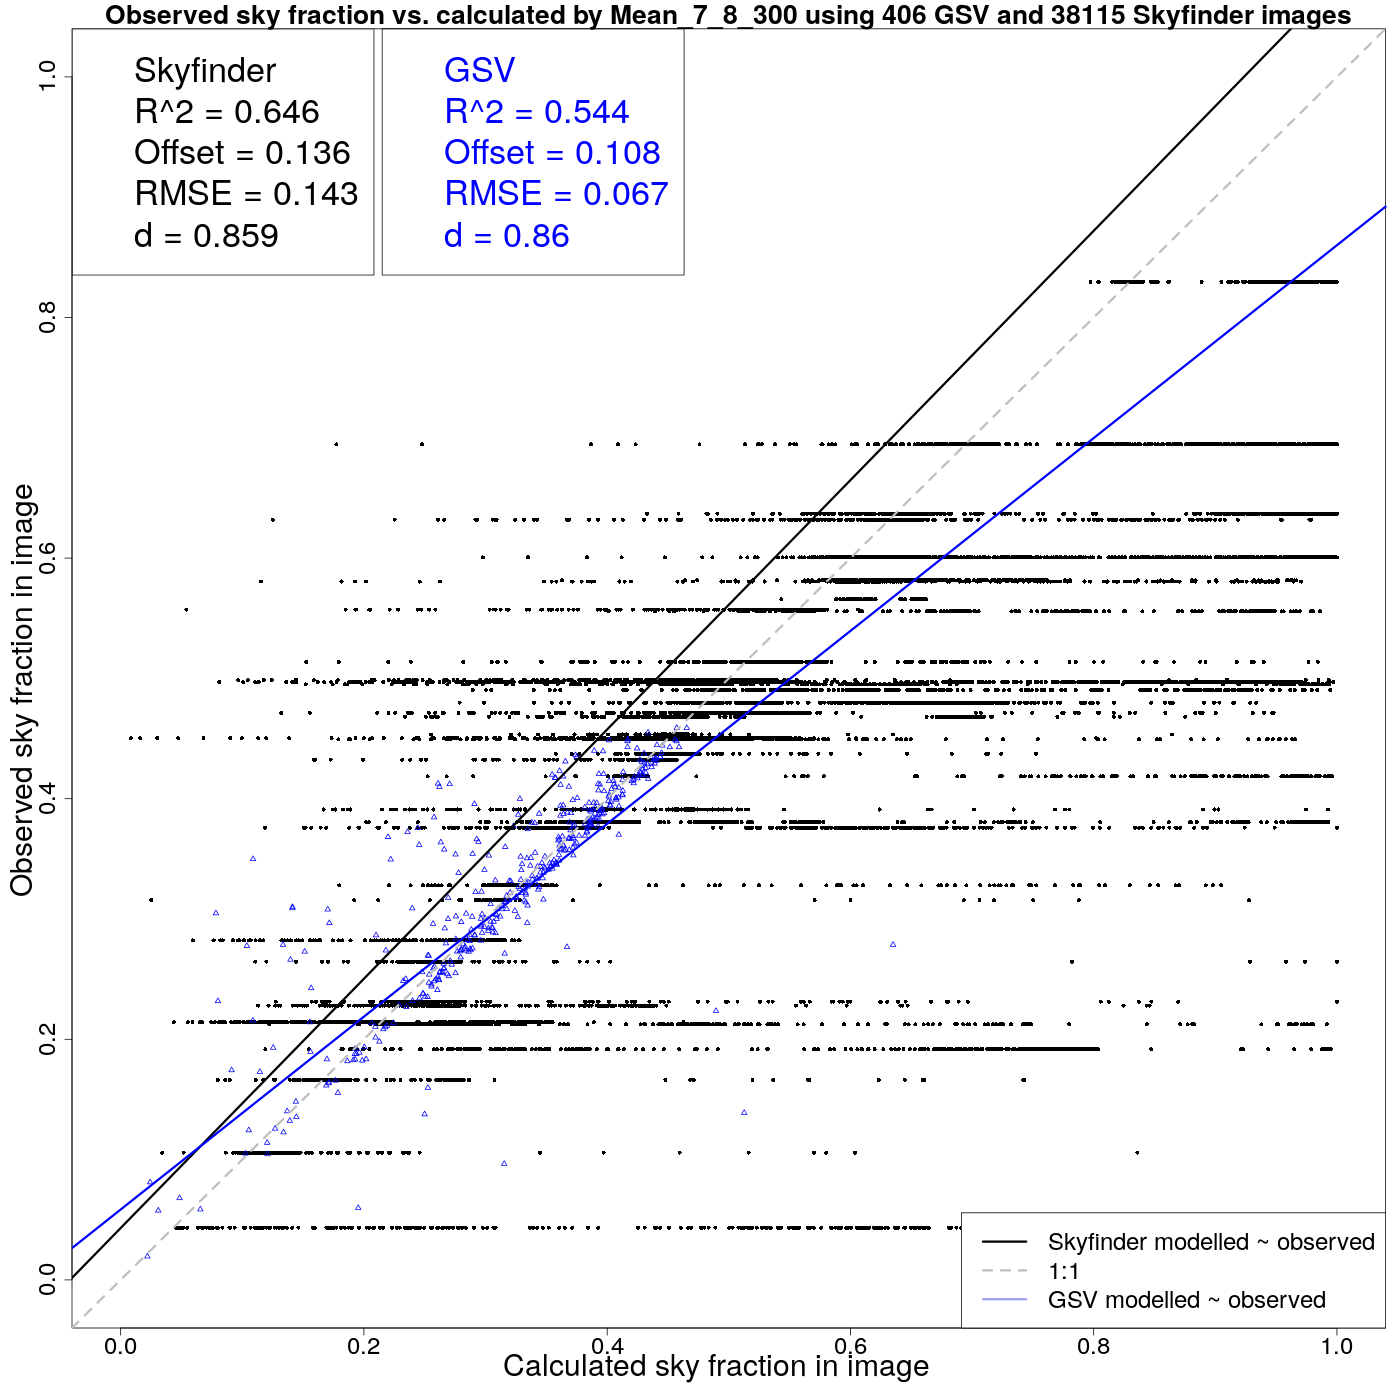
\includegraphics[scale=0.15,trim={8 10 5 0},clip]{Images/ErrorPlotsCombinedIndivMean_7_8_300.png}
\textbf{\scriptsize{b)}}\includegraphics[scale=0.15,trim={0 0 5 0},clip]{/home/kerryn/git/2018-03-MasterITProject/SkyViewDetection/SkyfinderEvaluationOutput/Plots/ErrorPlotsGSVandSMean_7_8_300_revised.png}
% R CMD BATCH /home/kerryn/git/2018-03-MasterITProject/SkyViewDetection/SkyfinderEvaluationOutput/Plots/scriptCombinedIndiv_Mean_7_8_300.R
% cp -u /home/kerryn/git/2018-03-MasterITProject/SkyViewDetection/SkyfinderEvaluationOutput/Plots/ErrorPlotsGSVandSMean_7_8_300.png /home/kerryn/git/2019-01-UrbanClimateSVF/Images/ErrorPlotsCombinedIndivMean_7_8_300.png
%\textbf{\scriptsize{c)}}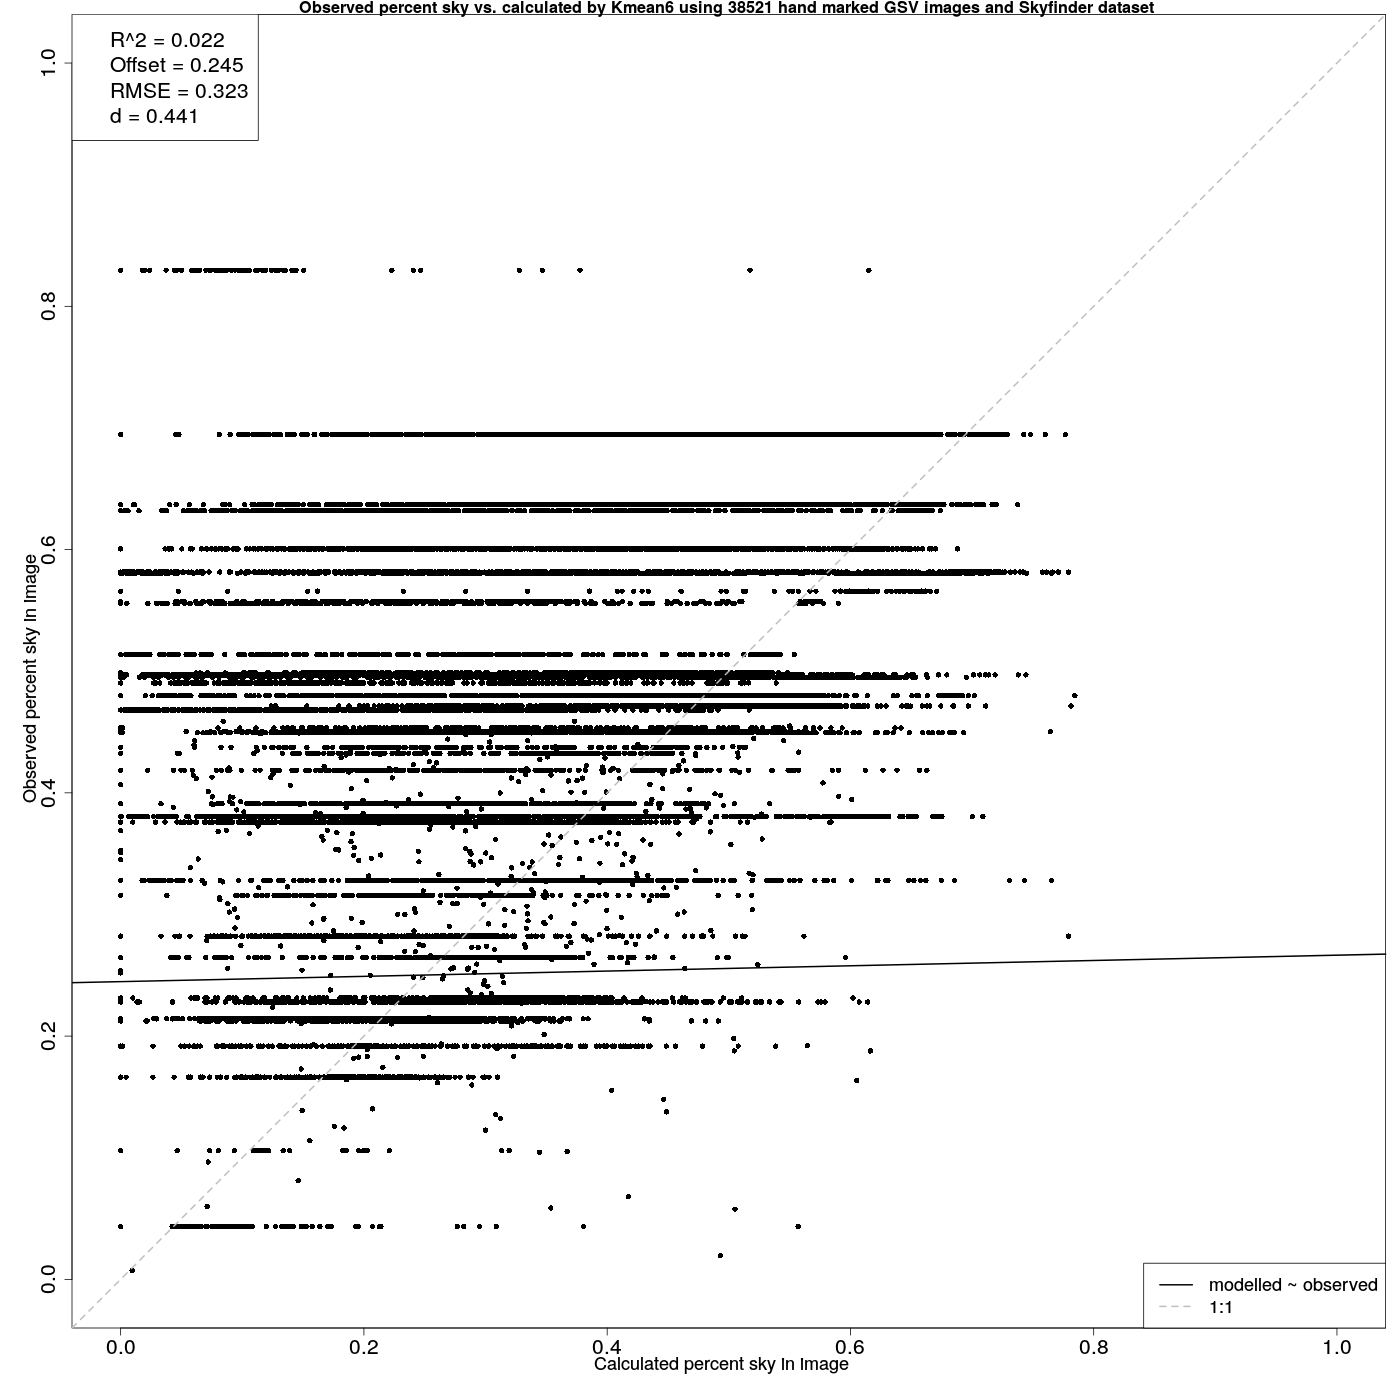
\includegraphics[scale=0.15,trim={8 10 5 0},clip]{Images/ErrorPlotsCombinedIndivKmean6.png}
\textbf{\scriptsize{c)}}\includegraphics[scale=0.15,trim={0 0 5 0},clip]{/home/kerryn/git/2018-03-MasterITProject/SkyViewDetection/SkyfinderEvaluationOutput/Plots/ErrorPlotsGSVandSKmean6_revised.png}
% R CMD BATCH /home/kerryn/git/2018-03-MasterITProject/SkyViewDetection/SkyfinderEvaluationOutput/Plots/scriptCombinedIndiv_Kmean6.R
% cp -u /home/kerryn/git/2018-03-MasterITProject/SkyViewDetection/SkyfinderEvaluationOutput/Plots/ErrorPlotsGSVandSKmean6.png /home/kerryn/git/2019-01-UrbanClimateSVF/Images/ErrorPlotsCombinedIndivKmean6.png
%\fbox{
%\textbf{\scriptsize{d)}}\includegraphics[scale=0.15,trim={8 10 5 0},clip]{Images/ErrorPlotsCombinedIndivSobel70.png}
\textbf{\scriptsize{d)}}\includegraphics[scale=0.15,trim={0 0 5 0},clip]{/home/kerryn/git/2018-03-MasterITProject/SkyViewDetection/SkyfinderEvaluationOutput/Plots/ErrorPlotsGSVandSSobel70_revised.png}
%}
% R CMD BATCH /home/kerryn/git/2018-03-MasterITProject/SkyViewDetection/SkyfinderEvaluationOutput/Plots/scriptCombinedIndiv_Sobel70.R
% cp -u /home/kerryn/git/2018-03-MasterITProject/SkyViewDetection/SkyfinderEvaluationOutput/Plots/ErrorPlotsGSVandSSobel70.png /home/kerryn/git/2019-01-UrbanClimateSVF/Images/ErrorPlotsCombinedIndivSobel70.png
%\caption{\textbf{Observed vs. calculated sky pixels using the a) Mean\_7\_6\_100, b) Mean\_7\_8\_300, c) K-mean\_6, and d) Sobel\_70 techniques on the 38,521 image combined dataset.} }
%\label{fig:errorallcombined}
\end{figure}
\clearpage %7

\begin{figure}
\centering
\textbf{\scriptsize{a)}}\includegraphics[trim = 0mm 0mm 0mm 0mm,clip,scale=0.14]{Images/13-0_Mean_7_8_300_tiles.png}
\textbf{\scriptsize{b)}}\includegraphics[trim = 0mm 0mm 0mm 0mm,clip,scale=0.14]{Images/13-3_Mean_7_6_100_tiles.png}
\textbf{\scriptsize{c)}}\includegraphics[trim = 0mm 0mm 0mm 0mm,clip,scale=0.14]{Images/13-5_K-mean_6_tiles.png}
\textbf{\scriptsize{d)}}\includegraphics[trim = 0mm 0mm 0mm 0mm,clip,scale=0.14]{Images/13-9_Sobel_70_tiles.png}
%\caption{\textbf{Selected imagery used for NN training for classifications 
%a) Mean\_7\_8\_300, b) Mean\_7\_6\_100, c) K-mean\_6, d) Sobel\_70.}}
%\label{fig:classImages}
\end{figure}
\clearpage %8


\begin{figure}
\centering
\textbf{\scriptsize{a)}}
%\includegraphics[scale=0.15,trim={8 10 5 0},clip]{Images/ErrorPlotsCNTK.png}
\includegraphics[scale=0.15,trim={0 0 5 0},clip]{/home/kerryn/git/2018-03-MasterITProject/SkyViewDetection/SkyfinderEvaluationOutput/Plots/ErrorPlotsCNTK13classesSkyfinderGSVEp249_revised.png}
% AnalyzeCNTKResults.java
% R CMD BATCH /home/kerryn/git/2018-03-MasterITProject/SkyViewDetection/SkyfinderEvaluationOutput/Plots/scriptCNTK_13classesSkyfinderGSVEp249.R
% cp -u /home/kerryn/git/2018-03-MasterITProject/SkyViewDetection/SkyfinderEvaluationOutput/Plots/ErrorPlotsCNTK13classesSkyfinderGSVEp249_2.png /home/kerryn/git/2019-01-UrbanClimateSVF/Images/ErrorPlotsCNTK.png 
\textbf{\scriptsize{b)}}
\includegraphics[scale=0.15,trim={0 0 5 0},clip]{/home/kerryn/git/2018-03-MasterITProject/SkyViewDetection/SkyfinderEvaluationOutput/Plots/ErrorPlotsGSVandSSobel70val_revised.png}
% AnalyzeResultsForGSVIndivTechniques2.java
% String imageSuffix= "Sobel70";
% R CMD BATCH /home/kerryn/git/2018-03-MasterITProject/SkyViewDetection/SkyfinderEvaluationOutput/Plots/scriptCombinedIndivVal_Sobel70.R
%  cp -u /home/kerryn/git/2018-03-MasterITProject/SkyViewDetection/SkyfinderEvaluationOutput/Plots/ErrorPlotsGSVandSSobel70val.png  /home/kerryn/git/2019-01-UrbanClimateSVF/Images/ErrorPlotsGSVandSSobel70val.png 
%\textbf{\scriptsize{c)}}\includegraphics[scale=0.15,trim={0 0 5 0},clip]{Images/ErrorPlots2FloodfillValidation.png}
\textbf{\scriptsize{c)}}\includegraphics[scale=0.15,trim={0 0 5 0},clip]{/home/kerryn/git/2018-03-MasterITProject/SkyViewDetection/SkyfinderEvaluationOutput/Plots/ErrorPlots2SplitFloodfillValidationSplit_revised.png}
% FloodfillEvaluation.java
% R CMD BATCH /home/kerryn/git/2018-03-MasterITProject/SkyViewDetection/SkyfinderEvaluationOutput/Plots/scriptFloodfillValidationSplitFloodfillValidationSplit.R
% cp -u /home/kerryn/git/2018-03-MasterITProject/SkyViewDetection/SkyfinderEvaluationOutput/Plots/ErrorPlots2SplitFloodfillValidationSplit.png /home/kerryn/git/2019-01-UrbanClimateSVF/Images/ErrorPlots2FloodfillValidation.png 
%\caption{\textbf{
%Results against the 9,636 validation images using a) our adaptive NN process, b) Benchmark 1: Sobel\_70, and c) Benchmark 2: Sobel/flood-fill combination.}}
%\label{fig:errorfloodall}
\end{figure}

\clearpage %9







\begin{figure}
\centering    
\textbf{\phantom{\textbf{\scriptsize{a)}}}}\includegraphics[scale=0.12]{/home/kerryn/git/2018-03-MasterITProject/SkyViewDetection/SkyfinderEvaluationOutput/GSV/mark_output_BigBuilding_3_6.0_100/panorama-JtVHmEl7WCiz1xJ0bcJpBg-1_seg.png} 
\textbf{\phantom{\textbf{\scriptsize{b)}}}}\includegraphics[scale=0.12]{/home/kerryn/git/2018-03-MasterITProject/SkyViewDetection/SkyfinderEvaluationOutput/GSV/mark_output_BigBuilding_7_6.0_100/panorama-JtVHmEl7WCiz1xJ0bcJpBg-1_seg.png} 
\textbf{\phantom{\textbf{\scriptsize{c)}}}}\includegraphics[scale=0.12]{/home/kerryn/git/2018-03-MasterITProject/SkyViewDetection/SkyfinderEvaluationOutput/GSV/mark_output_BigBuilding_5_7.0_210/panorama-JtVHmEl7WCiz1xJ0bcJpBg-1_seg.png} 
\textbf{\phantom{\textbf{\scriptsize{d)}}}}\includegraphics[scale=0.12]{/home/kerryn/git/2018-03-MasterITProject/SkyViewDetection/SkyfinderEvaluationOutput/GSV/mark_output_BigBuilding/panorama-JtVHmEl7WCiz1xJ0bcJpBg-1_seg.png} \scriptsize{1)}
\\
\textbf{\scriptsize{a)}}\includegraphics[scale=0.12]{/home/kerryn/git/2018-03-MasterITProject/SkyViewDetection/SkyfinderEvaluationOutput/GSV/mark_output_BigBuilding_3_6.0_100/panorama-JtVHmEl7WCiz1xJ0bcJpBg-1_ms_sky_mark.png} 
\textbf{\scriptsize{b)}}\includegraphics[scale=0.12]{/home/kerryn/git/2018-03-MasterITProject/SkyViewDetection/SkyfinderEvaluationOutput/GSV/mark_output_BigBuilding_7_6.0_100/panorama-JtVHmEl7WCiz1xJ0bcJpBg-1_ms_sky_mark.png} 
\textbf{\scriptsize{c)}}\includegraphics[scale=0.12]{/home/kerryn/git/2018-03-MasterITProject/SkyViewDetection/SkyfinderEvaluationOutput/GSV/mark_output_BigBuilding_5_7.0_210/panorama-JtVHmEl7WCiz1xJ0bcJpBg-1_ms_sky_mark.png} 
\textbf{\scriptsize{d)}}\includegraphics[scale=0.12]{/home/kerryn/git/2018-03-MasterITProject/SkyViewDetection/SkyfinderEvaluationOutput/GSV/mark_output_BigBuilding/panorama-JtVHmEl7WCiz1xJ0bcJpBg-1_ms_sky_mark.png} \scriptsize{2)}
\end{figure} 
\clearpage %10

\begin{figure}
\centering  
\textbf{\phantom{\textbf{\scriptsize{a)}}}}\includegraphics[width=3.50cm,height=1.75cm]{Images/mean/4880_7_6_100.png} 
\textbf{\phantom{\textbf{\scriptsize{b)}}}}\includegraphics[width=3.50cm,height=1.75cm]{Images/mean/4880_5_7_210.png} 
\textbf{\phantom{\textbf{\scriptsize{c)}}}}\includegraphics[width=3.50cm,height=1.75cm]{/home/kerryn/git/2018-03-MasterITProject/SkyViewDetection/SkyfinderEvaluationOutput/GSV2/mark_output_BigBuilding_7_6.0_100/0070_panorama_seg.png} 
\textbf{\phantom{\textbf{\scriptsize{d)}}}}\includegraphics[width=3.50cm,height=1.75cm]{/home/kerryn/git/2018-03-MasterITProject/SkyViewDetection/SkyfinderEvaluationOutput/GSV2/mark_output_BigBuilding_5_7.0_210/0070_panorama_seg.png} 
\scriptsize{1)}
\textbf{\textbf{\scriptsize{a)}}}\includegraphics[width=3.50cm,height=1.75cm]{Images/mean/4880_7_6_100_ms_sky_mark.png} 
\textbf{\textbf{\scriptsize{b)}}}\includegraphics[width=3.50cm,height=1.75cm]{Images/mean/4880_5_7_210_ms_sky_mark.png} 
\textbf{\scriptsize{c)}}\includegraphics[width=3.50cm,height=1.75cm]{/home/kerryn/git/2018-03-MasterITProject/SkyViewDetection/SkyfinderEvaluationOutput/GSV2/mark_output_BigBuilding_7_6.0_100/0070_panorama_ms_sky_mark.png} 
\textbf{\scriptsize{d)}}\includegraphics[width=3.50cm,height=1.75cm]{/home/kerryn/git/2018-03-MasterITProject/SkyViewDetection/SkyfinderEvaluationOutput/GSV2/mark_output_BigBuilding_5_7.0_210/0070_panorama_ms_sky_mark.png} 
\scriptsize{2)}

\end{figure} 

\clearpage %11


\begin{figure}
\centering  
%\includegraphics[scale=0.15]{Images/ErrorPlots1Combined.png}
\includegraphics[scale=0.15]{/home/kerryn/git/2018-03-MasterITProject/SkyViewDetection/SkyfinderEvaluationOutput/Plots/ErrorPlots2Reprocess2Theory_revised.png}
% AnalyzeResults2ReprocessTheory.java
% R CMD BATCH /home/kerryn/git/2018-03-MasterITProject/SkyViewDetection/SkyfinderEvaluationOutput/Plots/scriptReprocess2Theory.R
% cp -u /home/kerryn/git/2018-03-MasterITProject/SkyViewDetection/SkyfinderEvaluationOutput/Plots/ErrorPlots2Reprocess2Theory.png /home/kerryn/git/2019-01-UrbanClimateSVF/Images/ErrorPlots1Combined.png 
\end{figure} 

\clearpage %12

\begin{figure}
\centering 
\textbf{\scriptsize{a)}}\includegraphics[scale=0.41,trim={8 0 30 22},clip]{/home/kerryn/git/2018-03-MasterITProject/SkyViewDetection/SkyfinderEvaluationOutput/Plots/ResultsStatsBarPlot.png}
\textbf{\scriptsize{b)}}\includegraphics[scale=0.41,trim={8 0 30 22},clip]{/home/kerryn/git/2018-03-MasterITProject/SkyViewDetection/SkyfinderEvaluationOutput/Plots/ResultsStatsBarPlot2.png}
\textbf{\scriptsize{c)}}\includegraphics[scale=0.41,trim={8 0 30 22},clip]{/home/kerryn/git/2018-03-MasterITProject/SkyViewDetection/SkyfinderEvaluationOutput/Plots/ResultsStatsBarPlot3.png} 
\textbf{\scriptsize{d)}}\includegraphics[scale=0.41,trim={8 0 30 22},clip]{/home/kerryn/git/2018-03-MasterITProject/SkyViewDetection/SkyfinderEvaluationOutput/Plots/ResultsStatsBarPlot4.png}

\end{figure} 



\clearpage %13


\begin{figure}
\centering    
\textbf{\scriptsize{a)}}\includegraphics[scale=0.13]{Images/2/panorama-JtVHmEl7WCiz1xJ0bcJpBg-1_Sobel.png} \hfill%
\textbf{\scriptsize{b)}}\includegraphics[scale=0.13]{Images/2/panorama-JtVHmEl7WCiz1xJ0bcJpBg-1_Sobel_prob.png} \hfill%
\textbf{\scriptsize{c)}}\includegraphics[scale=0.13]{Images/2/panorama-JtVHmEl7WCiz1xJ0bcJpBg-1_Sobel_95_marked.png} \hfill%
\textbf{\scriptsize{d)}}\includegraphics[scale=0.13]{Images/2/panorama-JtVHmEl7WCiz1xJ0bcJpBg-1_Sobel_90_marked.png} 
\textbf{\scriptsize{e)}}\includegraphics[scale=0.13]{Images/2/panorama-JtVHmEl7WCiz1xJ0bcJpBg-1_Sobel_80_marked.png}\hfill% 
\textbf{\scriptsize{f)}}\includegraphics[scale=0.13]{Images/2/panorama-JtVHmEl7WCiz1xJ0bcJpBg-1_Sobel_70_marked.png}\hfill% 
\textbf{\scriptsize{g)}}\includegraphics[scale=0.13]{Images/2/panorama-JtVHmEl7WCiz1xJ0bcJpBg-1_Sobel_60_marked.png}\hfill% 
\textbf{\scriptsize{h)}}\includegraphics[scale=0.13]{Images/2/panorama-JtVHmEl7WCiz1xJ0bcJpBg-1_Sobel_50_marked.png} 
\textbf{\scriptsize{i)}}\includegraphics[scale=0.14]{/home/kerryn/git/2018-03-MasterITProject/SkyViewDetection/SkyfinderEvaluationOutput/19106/Examples/20130902_123654_Sobel.png} \hfill%
\textbf{\scriptsize{j)}}\includegraphics[scale=0.14]{/home/kerryn/git/2018-03-MasterITProject/SkyViewDetection/SkyfinderEvaluationOutput/19106/Examples/20130902_123654_Sobel_prob.png} \hfill%
\textbf{\scriptsize{k)}}\includegraphics[scale=0.14]{/home/kerryn/git/2018-03-MasterITProject/SkyViewDetection/SkyfinderEvaluationOutput/19106/Examples/20130902_123654_Sobel_95_marked.png} \hfill%
\textbf{\scriptsize{l)}}\includegraphics[scale=0.14]{/home/kerryn/git/2018-03-MasterITProject/SkyViewDetection/SkyfinderEvaluationOutput/19106/Examples/20130902_123654_Sobel_90_marked.png} 

\textbf{\scriptsize{m)}}\includegraphics[scale=0.14]{/home/kerryn/git/2018-03-MasterITProject/SkyViewDetection/SkyfinderEvaluationOutput/19106/Examples/20130902_123654_Sobel_80_marked.png} \hfill%
\textbf{\scriptsize{n)}}\includegraphics[scale=0.14]{/home/kerryn/git/2018-03-MasterITProject/SkyViewDetection/SkyfinderEvaluationOutput/19106/Examples/20130902_123654_Sobel_70_marked.png} \hfill%
\textbf{\scriptsize{o)}}\includegraphics[scale=0.14]{/home/kerryn/git/2018-03-MasterITProject/SkyViewDetection/SkyfinderEvaluationOutput/19106/Examples/20130902_123654_Sobel_60_marked.png} \hfill%
\textbf{\scriptsize{p)}}\includegraphics[scale=0.14]{/home/kerryn/git/2018-03-MasterITProject/SkyViewDetection/SkyfinderEvaluationOutput/19106/Examples/20130902_123654_Sobel_50_marked.png} 

%\caption{\bf  Results of Sobel operator/hybrid probability model, showing a) Sobel operator gradient image, b) resulting probability predictions, c) Sobel\_50, d) Sobel\_60, e) Sobel\_70, f) Sobel\_80, g) Sobel\_90, and h) Sobel\_95.}    
 %\label{fig:sobolresults}  
\end{figure} 

\clearpage %14

\begin{figure}
\centering    
%\textbf{a)}\includegraphics[scale=0.20]{Images/2/Cloudy/panorama-JtVHmEl7WCiz1xJ0bcJpBg-1_cropped.png} 
\textbf{\scriptsize{a)}}\includegraphics[scale=0.17]{Images/2/Cloudy/panorama-JtVHmEl7WCiz1xJ0bcJpBg-1_clustered6.png} 
\textbf{\scriptsize{b)}}\includegraphics[scale=0.17]{Images/2/Cloudy/panorama-JtVHmEl7WCiz1xJ0bcJpBg-1_HLS6.png} 
\textbf{\scriptsize{c)}}\includegraphics[scale=0.17]{Images/2/Cloudy/{panorama-JtVHmEl7WCiz1xJ0bcJpBg-1_sky_mark0.4}.png} 
\textbf{\scriptsize{d)}}\includegraphics[scale=0.17]{/home/kerryn/git/2018-03-MasterITProject/SkyViewDetection/SkyfinderEvaluationOutput/19106/Examples/20130902_123654_clustered6.png} 
\textbf{\scriptsize{e)}}\includegraphics[scale=0.17]{/home/kerryn/git/2018-03-MasterITProject/SkyViewDetection/SkyfinderEvaluationOutput/19106/Examples/20130902_123654_HLS6.png} 
\textbf{\scriptsize{f)}}\includegraphics[scale=0.17]{/home/kerryn/git/2018-03-MasterITProject/SkyViewDetection/SkyfinderEvaluationOutput/19106/Examples/{20130902_123654_sky_mark0.4}.png} 
%\caption{\bf  Results of K-means clustering and HSL color filtering (K-mean\_6), showing a) K-means clustered image, b) HSL intermediate image, and c) final marked image.}    
% \label{fig:kmeansresults}  
\end{figure} 

\clearpage %15
\begin{figure}
\centering    
\textbf{\phantom{\textbf{\scriptsize{a)}}}}\includegraphics[scale=0.12]{/home/kerryn/git/2018-03-MasterITProject/SkyViewDetection/SkyfinderEvaluationOutput/GSV/mark_output_BigBuilding_3_6.0_100/panorama-JtVHmEl7WCiz1xJ0bcJpBg-1_seg.png} 
\textbf{\phantom{\textbf{\scriptsize{b)}}}}\includegraphics[scale=0.12]{/home/kerryn/git/2018-03-MasterITProject/SkyViewDetection/SkyfinderEvaluationOutput/GSV/mark_output_BigBuilding_7_6.0_100/panorama-JtVHmEl7WCiz1xJ0bcJpBg-1_seg.png} 
%\textbf{\phantom{\textbf{\scriptsize{c)}}}}\includegraphics[scale=0.12]{/home/kerryn/git/2018-03-MasterITProject/SkyViewDetection/SkyfinderEvaluationOutput/GSV/mark_output_BigBuilding_5_7.0_210/panorama-JtVHmEl7WCiz1xJ0bcJpBg-1_seg.png} 
\textbf{\phantom{\textbf{\scriptsize{c)}}}}\includegraphics[scale=0.12]{/home/kerryn/git/2018-03-MasterITProject/SkyViewDetection/SkyfinderEvaluationOutput/19106/Examples/BB5_20130902_123654_seg.png} 
%\textbf{\phantom{\textbf{\scriptsize{d)}}}}\includegraphics[scale=0.12]{/home/kerryn/git/2018-03-MasterITProject/SkyViewDetection/SkyfinderEvaluationOutput/GSV/mark_output_BigBuilding/panorama-JtVHmEl7WCiz1xJ0bcJpBg-1_seg.png} \scriptsize{1)}
\textbf{\phantom{\textbf{\scriptsize{d)}}}}\includegraphics[scale=0.12]{/home/kerryn/git/2018-03-MasterITProject/SkyViewDetection/SkyfinderEvaluationOutput/19106/Examples/BB_20130902_123654_seg.png} \scriptsize{1)}
\\
\textbf{\scriptsize{a)}}\includegraphics[scale=0.12]{/home/kerryn/git/2018-03-MasterITProject/SkyViewDetection/SkyfinderEvaluationOutput/GSV/mark_output_BigBuilding_3_6.0_100/panorama-JtVHmEl7WCiz1xJ0bcJpBg-1_ms_sky_mark.png} 
\textbf{\scriptsize{b)}}\includegraphics[scale=0.12]{/home/kerryn/git/2018-03-MasterITProject/SkyViewDetection/SkyfinderEvaluationOutput/GSV/mark_output_BigBuilding_7_6.0_100/panorama-JtVHmEl7WCiz1xJ0bcJpBg-1_ms_sky_mark.png} 
%\textbf{\scriptsize{c)}}\includegraphics[scale=0.12]{/home/kerryn/git/2018-03-MasterITProject/SkyViewDetection/SkyfinderEvaluationOutput/GSV/mark_output_BigBuilding_5_7.0_210/panorama-JtVHmEl7WCiz1xJ0bcJpBg-1_ms_sky_mark.png} 
\textbf{\scriptsize{c)}}\includegraphics[scale=0.12]{/home/kerryn/git/2018-03-MasterITProject/SkyViewDetection/SkyfinderEvaluationOutput/19106/Examples/BB5_20130902_123654_ms_sky_mark.png} 
%\textbf{\scriptsize{d)}}\includegraphics[scale=0.12]{/home/kerryn/git/2018-03-MasterITProject/SkyViewDetection/SkyfinderEvaluationOutput/GSV/mark_output_BigBuilding/panorama-JtVHmEl7WCiz1xJ0bcJpBg-1_ms_sky_mark.png} \scriptsize{2)}
\textbf{\scriptsize{d)}}\includegraphics[scale=0.12]{/home/kerryn/git/2018-03-MasterITProject/SkyViewDetection/SkyfinderEvaluationOutput/19106/Examples/BB_20130902_123654_ms_sky_mark.png} \scriptsize{2)}
\end{figure} 

\clearpage %16



%/home/kerryn/git/2018-03-MasterITProject/SkyViewDetection/SkyfinderEvaluationOutput/19106/Examples/

%20130902_123654_clustered6.png    
%20130902_123654_HLS6.png   
%20130902_123654_sky_mark0.4.png 
%
%20130902_123654_Sobel.png
%20130902_123654_Sobel_prob.png
%20130902_123654_Sobel_50_marked.png
%20130902_123654_Sobel_60_marked.png
%20130902_123654_Sobel_70_marked.png
%20130902_123654_Sobel_80_marked.png
%20130902_123654_Sobel_90_marked.png
%20130902_123654_Sobel_95_marked.png
%
%20130902_123654_300x300_only.png  

%20130902_123654_300x300.png       
%20130902_123654.jpg      
%20130902_123654_clustered12.png   
%20130902_123654_ms_sky_mark.png 
%20130902_123654_clustered14.png   
%20130902_123654_seg.png 
%20130902_123654_cropped.png       
%20130902_123654_sky_mark0.6.png  
%20130902_123654_HLS12.png         
%20130902_123654_sky_mark0.7.png 
%20130902_123654_HLS14.png         


\begin{figure}
\centering    
\textbf{\scriptsize{a)}}\includegraphics[scale=0.20]{Images/2/FloodfillInput.png}
\textbf{\scriptsize{b)}}\includegraphics[scale=0.20]{Images/2/FloodfillMiddle.png}
\textbf{\scriptsize{c)}}\includegraphics[scale=0.20]{Images/2/FloodfillOutput.png}

\textbf{\scriptsize{d)}}\includegraphics[scale=0.20]{/home/kerryn/git/2018-03-MasterITProject/ArianesFloodfill/temp_fisheyes_out2/canvas.png}
\textbf{\scriptsize{e)}}\includegraphics[scale=0.28]{/home/kerryn/git/2018-03-MasterITProject/ArianesFloodfill/temp_fisheyes_out2/canvas2.png}
\textbf{\scriptsize{f)}}\includegraphics[scale=0.20]{/home/kerryn/git/2018-03-MasterITProject/ArianesFloodfill/temp_fisheyes_out2/canvas3.png}

%\caption{\bf   Results of Sobel/flood-fill combination, showing a) original image (rescaled to 512x512), b) intermediate Sobel image, and c) final marked sky image.}    
% \label{fig:sobelflood}  
\end{figure} 
\clearpage %17

\begin{figure}
\centering    
\textbf{\scriptsize{a)}}\includegraphics[scale=0.13]{Images/2/panorama-JtVHmEl7WCiz1xJ0bcJpBg-1_Sobel.png} %\hfill%
\textbf{\scriptsize{e)}}\includegraphics[scale=0.13]{Images/2/panorama-JtVHmEl7WCiz1xJ0bcJpBg-1_Sobel_80_marked.png}%\hfill% 
\textbf{\scriptsize{~i)}}\includegraphics[scale=0.14]{/home/kerryn/git/2018-03-MasterITProject/SkyViewDetection/SkyfinderEvaluationOutput/19106/Examples/20130902_123654_Sobel.png} %\hfill%
\textbf{\scriptsize{m)}}\includegraphics[scale=0.14]{/home/kerryn/git/2018-03-MasterITProject/SkyViewDetection/SkyfinderEvaluationOutput/19106/Examples/20130902_123654_Sobel_80_marked.png} 
\textbf{\scriptsize{b)}}\includegraphics[scale=0.13]{Images/2/panorama-JtVHmEl7WCiz1xJ0bcJpBg-1_Sobel_prob.png} %\hfill%
\textbf{\scriptsize{f)}}\includegraphics[scale=0.13]{Images/2/panorama-JtVHmEl7WCiz1xJ0bcJpBg-1_Sobel_70_marked.png}%\hfill% 
\textbf{\scriptsize{~j)}}\includegraphics[scale=0.14]{/home/kerryn/git/2018-03-MasterITProject/SkyViewDetection/SkyfinderEvaluationOutput/19106/Examples/20130902_123654_Sobel_prob.png} %\hfill%
\textbf{\scriptsize{n)}}\includegraphics[scale=0.14]{/home/kerryn/git/2018-03-MasterITProject/SkyViewDetection/SkyfinderEvaluationOutput/19106/Examples/20130902_123654_Sobel_70_marked.png} 

\textbf{\scriptsize{c)}}\includegraphics[scale=0.13]{Images/2/panorama-JtVHmEl7WCiz1xJ0bcJpBg-1_Sobel_95_marked.png} %\hfill%
\textbf{\scriptsize{g)}}\includegraphics[scale=0.13]{Images/2/panorama-JtVHmEl7WCiz1xJ0bcJpBg-1_Sobel_60_marked.png}%\hfill% 
\textbf{\scriptsize{~k)}}\includegraphics[scale=0.14]{/home/kerryn/git/2018-03-MasterITProject/SkyViewDetection/SkyfinderEvaluationOutput/19106/Examples/20130902_123654_Sobel_95_marked.png} %\hfill%
\textbf{\scriptsize{o)}}\includegraphics[scale=0.14]{/home/kerryn/git/2018-03-MasterITProject/SkyViewDetection/SkyfinderEvaluationOutput/19106/Examples/20130902_123654_Sobel_60_marked.png} 

\textbf{\scriptsize{d)}}\includegraphics[scale=0.13]{Images/2/panorama-JtVHmEl7WCiz1xJ0bcJpBg-1_Sobel_90_marked.png} %\hfill%
\textbf{\scriptsize{h)}}\includegraphics[scale=0.13]{Images/2/panorama-JtVHmEl7WCiz1xJ0bcJpBg-1_Sobel_50_marked.png} %\hfill%
\textbf{\scriptsize{~l)}}\includegraphics[scale=0.14]{/home/kerryn/git/2018-03-MasterITProject/SkyViewDetection/SkyfinderEvaluationOutput/19106/Examples/20130902_123654_Sobel_90_marked.png} %\hfill%
\textbf{\scriptsize{p)}}\includegraphics[scale=0.14]{/home/kerryn/git/2018-03-MasterITProject/SkyViewDetection/SkyfinderEvaluationOutput/19106/Examples/20130902_123654_Sobel_50_marked.png} 

 %\label{fig:sobolresults}  
\end{figure} 

\clearpage %18














\begin{figure}
\centering
\textbf{\scriptsize{a)}}\includegraphics[scale=0.15,trim={0 0 5 0},clip]{/home/kerryn/git/2018-03-MasterITProject/SkyViewDetection/SkyfinderEvaluationOutput/Plots/ErrorPlots2Reprocess2Theory_revised.png}
\textbf{\scriptsize{b)}}\includegraphics[scale=0.15,trim={0 0 5 0},clip]{/home/kerryn/git/2018-03-MasterITProject/SkyViewDetection/SkyfinderEvaluationOutput/Plots/ErrorPlotsCNTK13classesSkyfinderGSVEp249_revised.png}
\\
\textbf{\scriptsize{c)}}
\includegraphics[scale=0.15,trim={0 0 5 0},clip]{/home/kerryn/git/2018-03-MasterITProject/SkyViewDetection/SkyfinderEvaluationOutput/Plots/ErrorPlotsGSVandSSobel70val_revised.png}
\textbf{\scriptsize{d)}}\includegraphics[scale=0.15,trim={0 0 5 0},clip]{/home/kerryn/git/2018-03-MasterITProject/SkyViewDetection/SkyfinderEvaluationOutput/Plots/ErrorPlots2SplitFloodfillValidationSplit_revised.png}
\end{figure}

\clearpage %19



\begin{figure}
\centering    

\raisebox{7\height}{\scriptsize{1)}}\includegraphics[scale=0.08]{Images/mean/4880_3_6_100.png} 
\includegraphics[scale=0.08]{Images/mean/4880_7_6_100.png} 
\includegraphics[scale=0.08]{Images/mean/4880_5_7_210.png} 
\includegraphics[scale=0.08]{Images/mean/4880_7_8_300.png}
\\ 
\raisebox{7\height}{\scriptsize{2)}}\includegraphics[scale=0.08]{Images/mean/4880_3_6_100_ms_sky_mark.png} 
\includegraphics[scale=0.08]{Images/mean/4880_7_6_100_ms_sky_mark.png} 
\includegraphics[scale=0.08]{Images/mean/4880_5_7_210_ms_sky_mark.png} 
\includegraphics[scale=0.08]{Images/mean/4880_7_8_300_ms_sky_mark.png} 
%\\
%\textbf{\phantom{\textbf{\scriptsize{c)}}}}\includegraphics[scale=0.12]{/home/kerryn/git/2018-03-MasterITProject/SkyViewDetection/SkyfinderEvaluationOutput/19106/Examples/BB5_20130902_123654_seg.png} 
%\textbf{\phantom{\textbf{\scriptsize{d)}}}}\includegraphics[scale=0.12]{/home/kerryn/git/2018-03-MasterITProject/SkyViewDetection/SkyfinderEvaluationOutput/19106/Examples/BB_20130902_123654_seg.png} \scriptsize{1)}
%\\
%\textbf{\scriptsize{c)}}\includegraphics[scale=0.12]{/home/kerryn/git/2018-03-MasterITProject/SkyViewDetection/SkyfinderEvaluationOutput/19106/Examples/BB5_20130902_123654_ms_sky_mark.png} 
%\textbf{\scriptsize{d)}}\includegraphics[scale=0.12]{/home/kerryn/git/2018-03-MasterITProject/SkyViewDetection/SkyfinderEvaluationOutput/19106/Examples/BB_20130902_123654_ms_sky_mark.png} \scriptsize{2)}
\\
\scriptsize{a)}\hfil
\scriptsize{b)}\hfil
\scriptsize{c)}\hfil
\scriptsize{d)}\hfil

\end{figure} 



\clearpage %20


\begin{figure}
\centering    

\raisebox{7\height}{\scriptsize{1)}}\includegraphics[scale=0.08]{Images/mean/4880_3_6_100.png} 
\includegraphics[scale=0.08]{Images/mean/4880_7_6_100.png} 
\includegraphics[scale=0.08]{Images/mean/4880_5_7_210.png} 
\includegraphics[scale=0.08]{Images/mean/4880_7_8_300.png}
\\ 
\raisebox{7\height}{\scriptsize{2)}}\includegraphics[scale=0.08]{Images/mean/4880_3_6_100_ms_sky_mark.png} 
\includegraphics[scale=0.08]{Images/mean/4880_7_6_100_ms_sky_mark.png} 
\includegraphics[scale=0.08]{Images/mean/4880_5_7_210_ms_sky_mark.png} 
\includegraphics[scale=0.08]{Images/mean/4880_7_8_300_ms_sky_mark.png} 
\\
\raisebox{5\height}{\scriptsize{3)}}\includegraphics[scale=0.12]{/home/kerryn/git/2018-03-MasterITProject/SkyViewDetection/SkyfinderEvaluationOutput/19106/Examples/BB3_20130902_123654_seg.png} \hfil
\includegraphics[scale=0.12]{/home/kerryn/git/2018-03-MasterITProject/SkyViewDetection/SkyfinderEvaluationOutput/19106/Examples/BB7_20130902_123654_seg.png} \hfil
\includegraphics[scale=0.12]{/home/kerryn/git/2018-03-MasterITProject/SkyViewDetection/SkyfinderEvaluationOutput/19106/Examples/BB5_20130902_123654_seg.png} \hfil
\includegraphics[scale=0.12]{/home/kerryn/git/2018-03-MasterITProject/SkyViewDetection/SkyfinderEvaluationOutput/19106/Examples/BB_20130902_123654_seg.png} 
\\
\raisebox{5\height}{\scriptsize{4)}}\includegraphics[scale=0.12]{/home/kerryn/git/2018-03-MasterITProject/SkyViewDetection/SkyfinderEvaluationOutput/19106/Examples/BB3_20130902_123654_ms_sky_mark.png} \hfil
\includegraphics[scale=0.12]{/home/kerryn/git/2018-03-MasterITProject/SkyViewDetection/SkyfinderEvaluationOutput/19106/Examples/BB7_20130902_123654_ms_sky_mark.png} \hfil
\includegraphics[scale=0.12]{/home/kerryn/git/2018-03-MasterITProject/SkyViewDetection/SkyfinderEvaluationOutput/19106/Examples/BB5_20130902_123654_ms_sky_mark.png} \hfil
\includegraphics[scale=0.12]{/home/kerryn/git/2018-03-MasterITProject/SkyViewDetection/SkyfinderEvaluationOutput/19106/Examples/BB_20130902_123654_ms_sky_mark.png} 
\\
\scriptsize{a)}\hfil
\scriptsize{b)}\hfil
\scriptsize{c)}\hfil
\scriptsize{d)}\hfil

\end{figure} 



\clearpage %21

\begin{figure}
\centering  
\raisebox{4.5\height}{\scriptsize{1)}}\includegraphics[width=3.50cm,height=1.75cm]{Images/mean/4880_7_6_100.png} 
\includegraphics[width=3.50cm,height=1.75cm]{Images/mean/4880_5_7_210.png} 
\includegraphics[width=3.50cm,height=1.75cm]{/home/kerryn/git/2018-03-MasterITProject/SkyViewDetection/SkyfinderEvaluationOutput/GSV2/mark_output_BigBuilding_7_6.0_100/0070_panorama_seg.png} 
\includegraphics[width=3.50cm,height=1.75cm]{/home/kerryn/git/2018-03-MasterITProject/SkyViewDetection/SkyfinderEvaluationOutput/GSV2/mark_output_BigBuilding_5_7.0_210/0070_panorama_seg.png} 
\raisebox{4.5\height}{\scriptsize{2)}}\includegraphics[width=3.50cm,height=1.75cm]{Images/mean/4880_7_6_100_ms_sky_mark.png} 
\includegraphics[width=3.50cm,height=1.75cm]{Images/mean/4880_5_7_210_ms_sky_mark.png} 
\includegraphics[width=3.50cm,height=1.75cm]{/home/kerryn/git/2018-03-MasterITProject/SkyViewDetection/SkyfinderEvaluationOutput/GSV2/mark_output_BigBuilding_7_6.0_100/0070_panorama_ms_sky_mark.png} 
\includegraphics[width=3.50cm,height=1.75cm]{/home/kerryn/git/2018-03-MasterITProject/SkyViewDetection/SkyfinderEvaluationOutput/GSV2/mark_output_BigBuilding_5_7.0_210/0070_panorama_ms_sky_mark.png} 
\\
\scriptsize{a)}\hfil
\scriptsize{b)}\hfil
\scriptsize{c)}\hfil
\scriptsize{d)}\hfil

\end{figure} 

\end{document}